%
% MpLtX --- a LaTeX Template for Modern Physics Lab
% Copyright (C) 2013 Modern Phys. Lab, School of Phys., Peking Univ.
%
%   MpLtX is a template for experiment report of Modern Physics Lab in
% Peking University. This template depends on the "revtex4.1" package from
% APS Journals <http://publish.aps.org/revtex/revtex-faq>
%
% To use this template, you should open the package download from APS Journals'
% website as above and follow instructions from the README file in the package.
%
% LaTeX is marvelous for math formulae composition. However, the script grammar
% is rather difficult to handle. Maybe at the beginning, it's convenient to
% generate a pretty document. The deeper you went, more weird grammar you got.
% Before you found out the whole fantesy-like world built by Knuth, Lamport and
% numerous contributors, you would get numerous strange errors unclearly
% reported by compiler.
%
% Anyway, a lot of people wish to find a general document system which is both
% easy to use and strong enough to conveniently DIY. Word is easy to use.
% However, Word can not produce perfect document in art --- the position and
% size are not well calculated. By the way, it's such a pain to do simple but
% repeating work in Word such as formating title, generate large data table
% and etc. These works can be easily done in LaTeX if you know a little about
% programming. HTML is a easy-to-use language to create static document. It is
% compatible on all the machines currently because all you need is a simple
% browser (Firefox, Chrome or IE). In HTML5, the latest version of HTML, you
% can do colorful presentation about the report. You can present dynamic
% figures to present your idea clearly. However, the biggest problem for HTML
% is that this never renders a beautiful math formula in a simple way. HTML
% indeed has a math engine named as MathML. But this guy is notorious for its
% unreadable script grammar. So HTML+TeX --- the project MathJax, becomes a
% candidate of our dream communication media or e-document form. However, it is
% still under development. If you are interested in Java, JLaTeXMath package may
% be also a proper one since it provides a LaTeX renderer in Java.
%
% This template is modified by students in Peking University.
%   I am Sun Sibai. Cao Chuanwu shared the draft on RenRen Network. However,
% the draft did not match the requirement at all. It seems that Cao Chuanwu
% did not modified the style from package. He just put the origin content
% into LaTeX format.
%   I changed the style to satisfy the format requirement and fixed some problem
% about the incompatibility within the packages.
%
% So, if you have suggestions, please improve this template with your power. We
% will be always glad to see our work useful, popular and wonderful!
%
% This template has been tested in TeXLive 2012 with the command:
% $ xelatex mpltx.tex
% compile twice.
%
% Anyone can modify this template, but don't forget to list the previous
% developers and add yourself in.
%
% Sun Sibai <niasw@pku.edu.cn>
% Cao Chuanwu <>
%
\RequirePackage{fixltx2e} %This package in CTeX is not compatible with revtex4-1
\documentclass[aps,pre,12pt,preprint,onecolumn,showpacs,showkeys]{revtex4-1}
\usepackage{ctex}
\usepackage{setspace,dcolumn}
\usepackage{subfig}
\usepackage{hyperref}
\usepackage{graphicx,psfrag,epsfig}
\usepackage[font=small,format=plain,labelfont=bf,textfont=it,justification=raggedright,singlelinecheck=false]{caption}
\usepackage{amsmath,amsfonts,amssymb,amsthm,bm,upgreek}
\usepackage{geometry}
\usepackage[mathscr]{eucal}
\usepackage{algorithm2e}
\usepackage{bookmark}
\usepackage{setspace}
\usepackage{subfig}

%\usepackage[style=alphabetic,maxnames=4,minnames=3,maxbibnames=99]{biblatex}
%\usepackage{background} %Waterstamp package
%\SetBgContents{...的实验报告} %Waterstamp to prevent copying
%\SetBgScale{5} %Waterstamp setting
\hypersetup{colorlinks=true}
\geometry{top=2.54cm,bottom=2.54cm,left=3cm,right=3cm}
\renewcommand\appendixname{附录}
\renewcommand\abstractname{摘要}
\renewcommand\tablename{表}
\renewcommand\figurename{图}
\makeatletter
\def\@pacs@name{\songti\zihao{-4}{\bf PACS码:}}
\def\@keys@name{\songti\zihao{-4}{\bf 关键词:}}
\def\Dated@name{日期:}
\def\Received@name{\zihao{-5}{接收} }
\def\Revised@name{\zihao{-5}{修订} }
\def\Accepted@name{\zihao{-5}{采纳} }
\def\Published@name{\zihao{-5}{发表} }
\makeatother
%\linespread{1}
\renewcommand{\labelenumi}{\alph{enumi}.}
\leftmargini=20mm

\begin{document}
\title{\songti\zihao{-2}\bf{机器学习在物理中的应用}\vspace{15mm}}
\author{\songti\zihao{4}北京大学物理学院2016级~~~~方永康\vspace{2mm}\\
\songti\zihao{4}北京大学物理学院2016级~~~~钱思天\vspace{2mm}}
\keywords{机器学习,神经网络,夸克-胶子等离子体,集体流}
%\email{email@pku.edu.cn; (86)152XXXXXXXX}

\begin{abstract}
\vspace{10mm}
\begin{spacing}{1.5}
\songti\zihao{-4}
本文首先介绍机器学习的概况,并且介绍了本文所用到的机器学习的方法,
包括监督式学习的神经网络(Artificial Neural Network)方法以及非监督式学习的主成分分析方法(Principal Component Analysis,PCA),贝叶斯展开(Bayesian Unfolding)。
之后介绍了在重离子碰撞领域内的研究课题,包括利用流系数以及二粒子关联函数分析重离子碰撞后产生的各向异性流,
相对论性重离子碰撞演化模型,以及重离子碰撞中的长程解关联行为。之后介绍了将机器学习的方法应用到这些课题中,包括在二粒子关联作为输入的情况下,
利用主成分分析以及神经网络的方法对是否存在各向异性流进行判断,利用神经网络对重离子碰撞演化方程进行拟合,利用神经网络完成探测器效率修正以及利用贝叶斯展开研究重离子碰撞长程关联行为。最终发现,
在训练数据足够充分的情况下,神经网络能够很好的区分出流事件与非流事件,并且利用PCA这一方法,
我们也发现机器能够找出流与非流事件之间的区别,而这也很有可能就是神经网络用于区分流与非流的依据;同时,神经网络可以对重离子碰撞方程给出快速的较好的拟合;利用贝叶斯展开,能够对重离子
碰撞中的长程关联行为进行一定的还原。
\end{spacing}
\end{abstract}
\maketitle


\section{机器学习}
近年来,随着机器学习的不断发展,其在很多领域显示出了自己强大的能力,例如在围棋上alphago战胜世界冠军李世石,在自动驾驶上逐渐发挥出巨大的作用等等。在物理方面,机器学习也显示出了它强大的能力,
例如利用PCA分析XY模型,从而使得机器能够自动区分相变\cite{PhysRevB.96.144432},
利用卷积神经网络(CNN)对粒子喷注(jet)图像进行分类\cite{PhysRevD.94.112002},利用神经网络求解薛定谔方程\cite{PhysRevA.96.042113}等。
\subsection{神经网络}
\subsubsection{总述}
神经网络来源于仿生学,是模仿生物神经网络而创建的新的方法。
实现其功能的基本单元为:神经元及神经元间的连接,激活函数,损失函数。
而一般的前馈神经网络的结构如图~\ref{fig:cnn} 所示。整个网络由许多包含很多
神经元的层组成,大体可以分为输入层,隐藏层和输出层。我们将数据输入作为输入层再
通过神经元的连接传入隐藏层,隐藏层可能有多个,并且相邻的两个隐藏层之间也通过神经元
相连接起来,最终将结果传递至输出层输出。
我们用最简单的前馈神经网络的层间连接来演示神经网络神经元间的连接,
对于相连的两层,我们假定前后两层分别为
$\alpha$、$\beta$层,前后两层分别有$n_{\alpha}$、$n_{\beta}$个神经元,并且
两层存储的数据由向量$\bm h^{\alpha}$、$\bm h^{\beta}$表示,如图~\ref{fig:cjlj} 所示。
因此$\beta$层神经元的数据可由式~\ref{eq:1} 表示。
\begin{equation}
h_{j}^{\beta}=f(\sum_{i=1}^{n_{\alpha}}W_{ji}h_{i}^{\alpha}+b_{j}) \label{eq:1}
\end{equation}
其中$h_{i}^{\alpha}$、$h_{j}^{\beta}$是$\alpha$、$\beta$层存储数据的向量$\bm h^{\alpha}$、$\bm h^{\beta}$
在第$i$、$j$个神经元上的分量,$W_{ji}$为权重参数,$b_{j}$为偏置参数,这两者一般就是神经网络
需要训练的参数,$f$为前面提及的激活函数,用于引入非线性效应。这就是一般神经网络神经元之间的连接。\par
经过层层连接,最终连接至输出层,在输出层将利用损失函数来判断网络的输出与真实结果之间的差,之后通过
反向传播算法,来拟合前面提到的权重参数与偏置参数,从而是网络获得接近真实值的输出,即网络训练完成。
一般而言,神经网络用于处理回归问题与分类问题,对于两种问题所用到的损失函数一般不相同。我们假定网络输出值
为$y^{p}$,真实结果为$y^{r}$,那么对于回归问题一般用平方损失函数~\ref{eq:2} ,对于分类问题一般用交叉熵损失函数~\ref{eq:3}。
\begin{align}
Loss(y^{p},y^{r})&=\|y^{p}-y^{r}\|^{2} \label{eq:2} \\
Loss(y^{p},y^{r})&=-\sum_{i}y_{i}^{r}lny_{i}^{p} \label{eq:3}
\end{align}
\par
\begin{figure}[htbp]
\centering
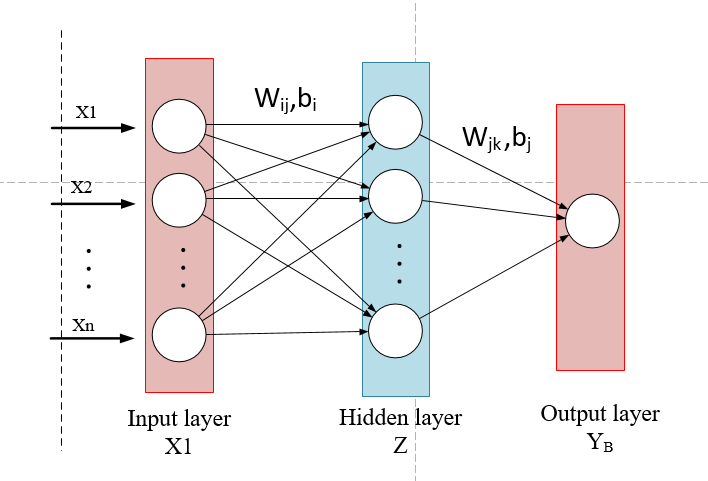
\includegraphics[width=80mm]{CNN}
\caption{\label{fig:cnn}%
此图表示了前馈神经网络的一般结构,数据从输出层输入,被传递
入隐藏层,最终通过输出层输出}
\end{figure}
\begin{figure}[htbp]
\centering
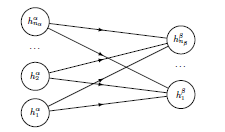
\includegraphics[width=80mm]{cjlj}
\caption{\label{fig:cjlj}%
此图表示了前馈神经网络层与层之间的联系}
\end{figure}
\begin{figure}[htbp]
\centering
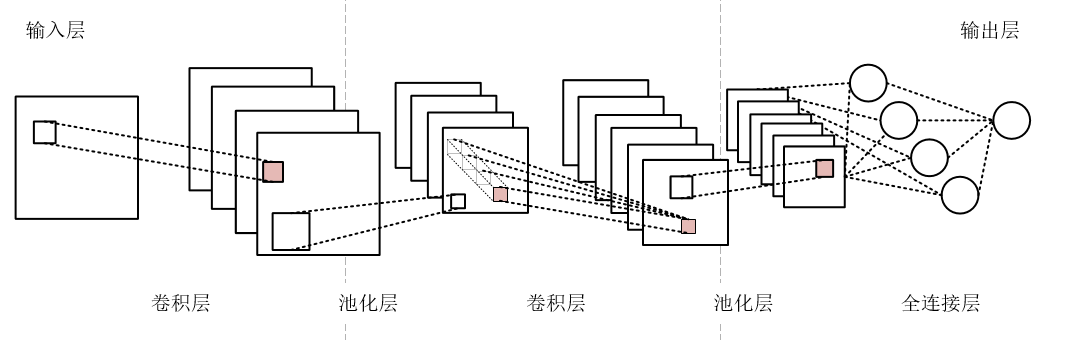
\includegraphics[width=80mm]{cnnn}
\caption{\label{fig:cnnn}%
此图表示了卷积神经网络的一般结构,其中较为特别的是卷积层与池化层}
\end{figure}
\begin{figure}[htbp]
\centering
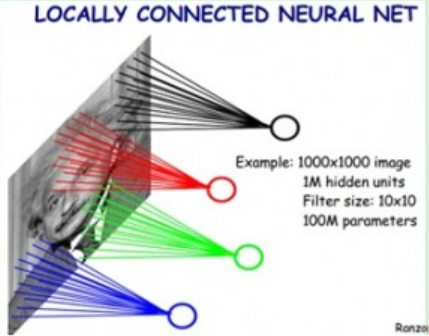
\includegraphics[width=80mm]{cnv}
\caption{\label{fig:cnv}%
此图表示了卷积层的工作模式}
\end{figure}
\begin{figure}[htbp]
\centering
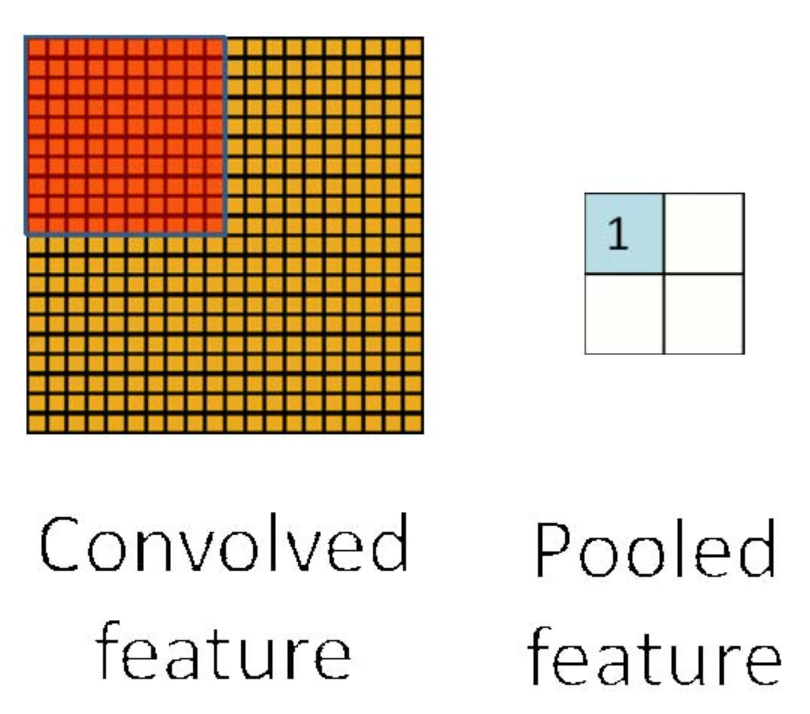
\includegraphics[width=80mm]{pool}
\caption{\label{fig:pool}%
此图表示了池化层的工作模式}
\end{figure}
\subsubsection{卷积神经网络}
传统的卷积神经网络(Convolutional Neural 
Network, CNN)是本文中将要涉及的一类神经网络,其基本结构如图~\ref{fig:cnnn} 所示。可以看到,与之前展示的前馈神经网络相比,二者基本一致,
只是对于卷积神经网络有两类特殊的层,即卷积层与池化层,下面将简要解释下。对于卷积层,如图~\ref{cnv} ,一个重要的思想就是共享参数。
前一层为爱因斯坦图像,后一层为四种颜色点所示的一层,这四个点
与前一层部分点相连,更合理的想法为有一个滤波器存储相关参数,其扫过前一层,按照类似前面所述的层与层间的
运算规则,会得到新一层,因此,新一层的所有神经元均通过此滤波器上的参数与前一层的部分神经元相连,因此在这两层之间实现了参数共享,
而这就是卷积层的工作原理,而此时如果选择多个滤波器,就可以得到对应于同一层的多个新层,这也就实现了多通道
,也就是图~\ref{fig:cnnn} 中所示的前后两层可能有不同的通道数。对于池化层,如图~\ref{fig:pool} 所示,
图中两层直接相连,前一层的红色区域与池化层的蓝色区域相对应,其余部分各自对应,然后对应的区域按一定的规则,例如:
仅取最大值或取平均值规则来得到下一层,得到的新层即为池化层,按所用规则对应为最大池或平均池。这两种层的优点在于,
卷积层能够提取出图像中的局部信息,池化层能够压缩数据,防止过拟合等等。
\subsubsection{贝叶斯神经网络}
贝叶斯神经网络(Bayesian Neural Network)是基于贝叶斯理论的人工神经网络结构,在面对小样本学习时有独特的优势。\par
当我们采用神经网络进行数据拟合时,贝叶斯公式有着如下表述:
\begin{equation}
    p(W | X, Y)=\frac{p(W) p(Y | X, W)}{p(Y | X)}
\end{equation}
式中,$W$代表网络中的参数,$(X,Y)$则是数据集数据,$X$代表输入,而$Y$代表输出。\par
因此,对于给定的数据集,$p(Y|X)$是给定的,而剩下的各项,$p(W)$是参数的先验分布,而$p(Y|X,W)$则代表了网络在给定参数$W$和输入$X$时获得的输出概率。\par
神经网络的一大应用场景是拟合复杂的映射,$p(W|X,Y)$的真实形式往往十分复杂。因此,在贝叶斯神经网络中,我们并不直接求解,而是通过一个参数化的分布
$q(W)$来逼近$p(W)$。\par
在信息论中,人们往往会采用KL散度(又称为相对熵)来描述两个分布的接近程度,对于我们的问题,有:
\begin{equation}
    \begin{aligned}
    KL(q||p)&=\int q(W)\log{\frac{q(W)}{p(W|X,Y)}}\\
    &=E_q[\log{\frac{q(W)}{p(W|X,Y)}}]
    \end{aligned}
\end{equation}
注意到KL散度并不是对称的,在我们的问题中,由于$p(W|X,Y)$的计算实际上还需要利用$q(W)$,因此采用如式的前向KL散度更符合信息论意义。同时,以$p(W|X,Y)$求期望操作也难以实现。\par
因此问题变为:
\begin{equation}
    \begin{aligned}
        \min_{q(W)}KL(q||p)&=\min_{q(W)}E_q[\log{\frac{q(W)}{p(W|X,Y)}}]\\
        &=\min_{q(W)}E_{q}[\log q(W)-\log p(W)-\log p(Y | X, W)+\log p(Y | X)]
        \end{aligned}
\end{equation}
下面讨论每一项的求解:
\begin{enumerate}
    \item $E_q[\cdot]$\par 根据$q(W)$求期望这一操作的实现可以通过根据$q(W)$进行大量采样求平均完成;
    \item $\log q(W)$\par 这一项可以根据$q(W)$的形式直接获得,一般来说,人们会选择W中各分量各自符合一个高斯分布;
    \item $\log p(W)$\par 这一项可以通过适当选取先验获得,一个通常的选择是高斯分布;
    \item $\log p(Y|X)$\par 对于特定的问题来说,这一项是常数,优化问题中可以不加考虑;
    \item $\log p(Y | X, W)$\par 这一项的意义是给定参数$W$与输入$X$下,输出$Y$的分布,由于我们取$W$各分量均为高斯分布,并认为可以足够接近真实分布,因此
    ,网络输出也应该是一个高斯分布,其期望值正是$X$对应的$Y_{pred}$,所以
    \begin{equation}
        p(Y | X, W)=\frac{1}{\sqrt{2 \pi} \sigma} \exp \left(\left(Y-Y_{p r e d}\right)^{T} \sigma_{-1}\left(Y-Y_{p r e d}\right)\right)
    \end{equation}
    式中$\sigma_{-1}$是可调参数,代表了高斯分布的标准差,通常的选择是与$p(W)$的先验保持一致。
\end{enumerate}
\begin{figure}[htbp]
\centering
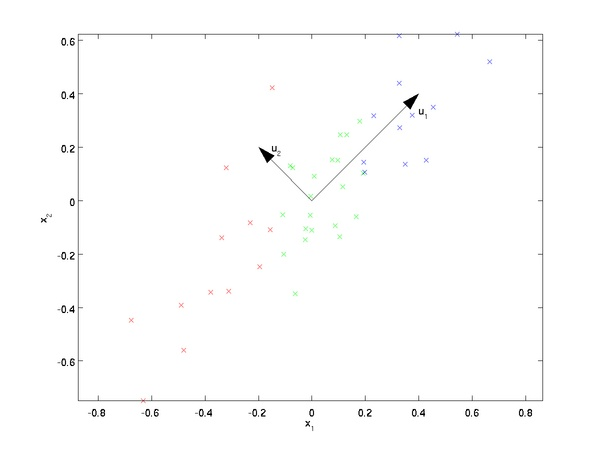
\includegraphics[width=80mm]{pca}
\caption{\label{fig:pca}%
此图表示了主成分分析的工作模式}
\end{figure}

\subsection{主成分分析}
主成分分析属于非监督式学习的范畴,下面将简要介绍一下其原理。\par
首先我们指出,我们得到的所有数据都是分布在一定的高维空间之中,但是我们的数据在初始给定的
这个空间的各个基上一般是相关的,主成分分析的思路即是选择一组新的基,使得数据在这些机上一般
是相互独立的。如图~\ref{fig:pca} 所示,初始数据是分布在\{$x_{1}$,$x_{2}$\}两个基构成的二维
平面内,可以看出,数据在这两个基上的分布是高度相关的,而主成分分析即是通过一定的数学手段找到一组新的
基\{$u_{1}$,$u_{2}$\},可以看出,数据在这两个基上的分布几乎是独立的。下面将简要介绍一下如何实现这一变换。\par
假设我们的数据为$n$个$m$维数据,记为向量$\bm x_{i}$($i=1,2,\cdots,n$),这就表示$n$个具有$m$个特征的样本。
因此,我们可以得到样本的均值为:
$\bm{\bar{x}}=\sum_{i=1}^{n}\bm{x_{i}}$,之后我们可以得到数据在这$m$个特征维度上的
协方差为$Cov=\sum_{i=1}^{n}\bm{(x_{i}-\bar{x})(x_{i}-\bar{x})}^{T}$,这样得到的是一个$m*m$维的协方差矩阵,我们
可以对这个矩阵进行对角化,这样会得到一组新的基,不难理解,数据在新的基上的分布是相互独立的,并且,本征值越大,表明数据
在这个基方向上分布的差异性最大,对我们也越有意义,挑出本征值较大的几个基方向,也就是这组数据的主成分。至此,我们便实现
了主成分分析。
\subsection{贝叶斯展开}
贝叶斯展开,是一种数据驱动的,利用贝叶斯公式对分布进行重建的无监督学习方法,在高能物理实验与核物理实验中有着广泛的应用。\par
对于某一观测量的分布(或计数),我们都可以(事实上也不得不)利用离散的向量$\vec{d}$来进行刻画,其中,分量$d_i$表示了落入第$i$区间的概率(或计数)。
类似的,联合分布概率(或计数)可以用矩阵$A$来刻画,分量$A_{ij}$表示落入区间$(i,j)$的概率(或分布),通过对联合分布矩阵不同维度的归一化,还可以得到条件概率矩阵。\par
因此,如果我们以$c$标注源(cause)分布,而用$e$标注响应(effect)分布,那么,著名的贝叶斯公式
\begin{equation}p(\tilde{c}_i|\tilde{e}_j)=\frac{p(\tilde{e}_j|\tilde{c}_i)p(\tilde{c}_i)}{\int p(\tilde{e}_j|\tilde{c})p(\tilde{c})d\tilde{c}}\end{equation}
可以写成离散形式:
\begin{equation}M_{ji}=\frac{A_{ij}c_j}{\sum_{k}A_{ik}c_k}\end{equation}
式中,$A_{ij}$与$M_{ji}$分别是两条件分布的离散形式,而$\vec{c},\vec{e}$则是连续分布$\tilde{c},\tilde{e}$的离散形式。\par
在实验上,我们可以直接获得$\vec{e}$,同时根据不同的需求构造$A_{ij}$,例如,在高能实验领域中,可以利用GEANT对探测器进行模拟,进而获得
基于模型的响应矩阵$A_{ij}$.
获得了$A_{ij}$与$\vec{e}$后,可以构造如下的迭代流程:\par
\begin{algorithm}
    \SetAlgoLined
    \KwData{$A_{ij},\vec{e}$}
    \KwResult{$\hat{\vec{c}}$: $\vec{c}$的一个估计值}
    为$\vec{c}$选取适合的先验分布$\vec{c}_0$并决定迭代次数$I$\;
    \For{iter=1:I}{
        $M^{iter}_{ji}=\frac{A_{ij}c^{iter-1}_j}{\sum_{k}A_{ik}c^{iter-1}_k}$\;
        $c^{iter}_j=\sum_{k}M^{iter}_{jk}e_k$\;
    }
    $\hat{\vec{c}}$=$\vec{c}^{I}$\;
    \caption{贝叶斯展开的迭代算法}
\end{algorithm}
这个迭代步骤最终将会收敛到贴近真实源分布附近,但一般来说,人们并不会令迭代次数过分大,以避免过多迭代带来的误差累积。
\begin{figure}[htbp]
\centering
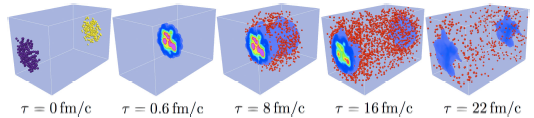
\includegraphics[width=140mm]{QGP}
\caption{\label{fig:QGP}%
此图表示了相对论性重离子碰撞产生QGP的过程}
\end{figure}
\begin{figure}[htbp]
\centering
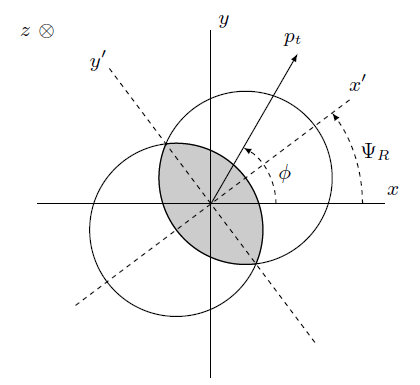
\includegraphics[width=80mm]{hz}
\caption{\label{fig:hz}%
核子相碰示意图}
\end{figure}
\section{相对论重离子碰撞简介}
在相对论性重离子碰撞过程中,由于其生成的高密度环境,可能使得夸克和
胶子接触禁闭,形成QGP,整个过程可由图~\ref{fig:QGP} 表示\cite{2013PhDT........31Q}。
可以看出,在碰撞后的零点几飞米时间内,出现QGP,在
碰撞后的几飞米时间内,会重新生成新的粒子,最终,探测器可以探测到最后的
粒子分布。为了研究QGP的性质,但受限于其存在时间极短,空间尺度极小等特点,
需要通过最终的粒子分布来间接的推知QGP的性质。现在认为,QGP的性质与流体
相似,都有很强的集体行为,而采用流体的方法来研究QGP的性质的方法即为集体流方法,
也可以称为各向异性流方法\cite{2010LanB...23..240H}。
\subsection{定义}
如图~\ref{fig:hz} 所示,表示的式在垂直粒子数方向上两核子相碰的相关物理量,
$x-y-z$为实验室坐标系,$x^{'}-y^{'}$为两核子中心连线方向坐标系,其中$x^{'}$与$x$之间
的夹角为$\psi_{R}$,被称为反应平面角(event plane angle)。$p_{t}$表示最终形成的粒子
的动量在$x-y$平面上的分量,$\phi$为$p_{t}$在$x-y$平面内的方位角,赝快度$\eta=\operatorname¡{arctanh}(\frac{p_{z}}{|p|})$
用于表示粒子在$z$方向上分布性质。因此,粒子的产额可用式~\ref{eq:4} 表示\cite{PhysRevC.58.1671}。
\begin{equation}
E\frac{d^{3}N}{dp^{3}}=\frac{1}{2\pi}\frac{d^{2}N}{p_{t}dp_{t}d\eta}(1+\sum_{i=1}^{\infty}2v_{n}cos(n(\phi-\psi_{R}))) \label{eq:4}
\end{equation}
其中,傅里叶展开系数$v_{n}$用于表示各阶各向异性流的强度,其中$v_{2}$为椭圆流,$v_{3}$为三角流。通过研究
各阶流,既可以间接研究碰撞时的相关物理过程。研究各阶流的方法有很多,一般有事件平面法,二粒子和多粒子关联法,
子事件方法等。本文在研究时用到的方法是二粒子关联函数法,下面简要介绍下。
\subsection{二粒子关联函数法}
二粒子关联函数的定义如式~\ref{eq:5} 所示\citet{PhysRevC.96.024908,PhysRevLett.116.172302},其中自变量$\Delta\phi$、$\Delta\eta$分别表示两粒子的方位角$\phi$与
赝快度$\eta$的差值。同时$S(\Delta\phi,\Delta\eta)$是同一碰撞事件所有粒子对在($\Delta\phi$,$\Delta\eta$)空间
上的分布,其中包含了所有的关联,即既包含了物理上的关联,也包含了非物理的关联。而$B(\Delta\phi,\Delta\eta)$是背景
的分布,其来源于两个不同碰撞事件的粒子对在($\Delta\phi$,$\Delta\eta$)空间上的分布,其中只包含非物理的关联。同时
要考虑到涨落的影响,因此在实验上,$S(\Delta\phi,\Delta\eta)$和$B(\Delta\phi,\Delta\eta)$将进行大量事件平均后,
最终得到在事件平均下的二粒子关联函数$C(\Delta\phi,\Delta\eta)$。
\begin{equation}
C(\Delta\phi,\Delta\eta)=\frac{\sum_{events}S(\Delta\phi,\Delta\eta)}{\sum_{events}B(\Delta\phi,\Delta\eta)} \label{eq:5}
\end{equation}
\par
如图~\ref{fig:fnf} 所示\citet{PhysRevC.96.024908},左图表示的是非流事件的示意图,右图表示的是流事件的示意图。可以看到非流时间仅有在$\Delta\phi=0,\Delta\eta=0$
处的尖峰结构以及在$\Delta\phi=\pi$处的脊结构,而对于流事件,还存在$\Delta\phi=0$处的脊结构,这被称为流事件中的双脊结构,
而这也是区分流与非流事件的一个很重要的特征。
\begin{figure}[htbp]
\centering
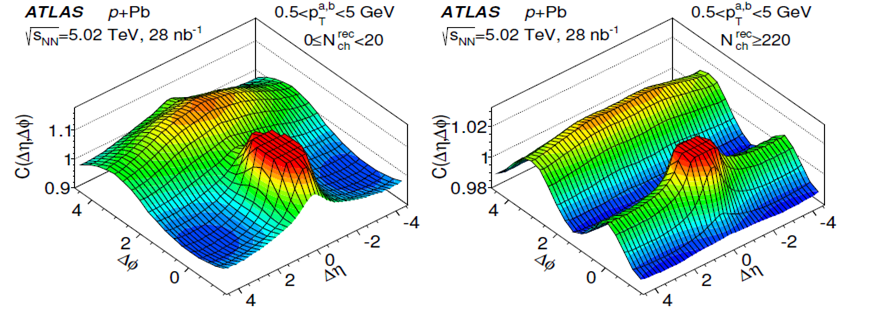
\includegraphics[width=140mm]{fnf}
\caption{\label{fig:fnf}%
流与非流的二粒子关联函数示意图,左图表示的是非流的图像,右图表示的是流的图像}
\end{figure}
\subsection{相对论性重离子碰撞的一种建模方式}
在相对论性重离子碰撞中,有许多成功的模型,都可以与实验数据保持良好的一致性。而在我们的课题研究中,主要采用了TRENTO+VISHNU的联合建模方式。
\subsubsection{逐事件约化厚度核拓扑模型(TRENTO)}
逐事件约化厚度核拓扑模型,是一个简约,计算迅速的相对论性核碰撞(质子对撞,质子重核对撞,重核对撞)初态模型。
\par
相对论性重离子碰撞领域中已经存在许多成功的初态模型,动力学模型有基于色玻璃凝聚有效场论的基于碰撞参数的Glasma模型(IP-Glasma),静态模型则有蒙特卡洛Glauber模型(MC-Glauber),都各自成功的解释了实验数据。而逐事件约化厚度核拓扑模型,则可以通过模型参数的选取,分别贴近不同的初态模型。
\par
假设一对碰撞核子A,B,沿着z轴碰撞,同时,记$\rho_{A,B}^{part}$为参与碰撞的非弹性碰撞部分。由此,每个碰撞核子的厚度可以用参与部分表示出来:
\begin{equation}
    T_{A,B}(x,y)=\int dz \rho_{A,B}^{part}(x,y,z)
\end{equation}
厚度函数的选取会在之后简述。\par
一旦拥有了厚度函数,依照如下的原则,我们就可以构造熵作为初态。
\begin{enumerate}
    \item 熵的产生来自于A和B的密度重合;
    \item 存在一个标量场$f(T_A,T_B)$,将厚度转化成熵。
\end{enumerate}
具体来说,首先,标量场$f$应当正比于在中快度区间内流体热力学演化时刻产生的熵。
\begin{equation}
    f\propto dS/dy|_{\tau=\tau_0}
\end{equation}
它应当给出一个有效的对碰撞早期动力学的描述:并不一定来自于第一性原理的计算,但要满足物理限制。
\par
从来自相对论性重离子对撞机的超中心对撞数据,可以得出核子碰撞应该满足规模不变的性质:
\begin{equation}
    f(cT_A,cT_B)=cf(T_A,T_B)
\end{equation}
也就是说,N个1对1的碰撞的效应总和,在数学上应该和一个N对N的碰撞效应相同。\par
因此,可选取如下的场$f$:
\begin{equation}
    f=T_R(p;T_A,T_B)=(\frac{T^p_A+T^P_B}{2})^{1/p}
\end{equation}
称为约化厚度。\par
约化厚度场$f$可视为广义上的均值,其取值可以随着无量纲参数$p$的变化,在$T_A$和$T_B$的最大值和最小值之间变化。
\begin{equation}
T_{R}=\left\{\begin{array}{ll}{\max \left(T_{A}, T_{B}\right)} & {p \rightarrow+\infty} \\ 
{\left(T_{A}+T_{B}\right) / 2} & {p=+1, \text { (算数平均数) }} \\ 
{\sqrt{T_{A} T_{B}}} & {p\to0, \quad \text { (几何平均数) }} \\ 
{2 T_{A} T_{B} /\left(T_{A}+T_{B}\right)} & {p=-1, \text { (调和平均数) }} \\ 
{\min \left(T_{A}, T_{B}\right)} & {p \rightarrow-\infty}\end{array}\right.
\end{equation}
从物理意义上看,$p$的取值是不同的熵产生机制的反应。\par
对于碰撞粒子厚度的计算可按照如下流程:\par
考虑一对碰撞质子A、B,碰撞参数为b,碰撞参数处在x轴方向:
\begin{equation}
    \rho_{A,B}=\rho_{p}(x\pm b/2,y,z)
\end{equation}
如果假设密度在碰撞方向上的积分是收敛的或者至少可以计算,那么可以计算出碰撞的概率:
\begin{equation}
    P_{\mathrm{coll}}=1-\exp \left[-\sigma_{g g} \int d x d y \int d z \rho_{A} \int d z \rho_{B}\right]
\end{equation}
指数里的积分是重叠部分的积分,而$\sigma_{gg}$是有效核子碰撞界面,其取值应被选取为满足总碰撞截面$\sigma_{NN}$。
\par
碰撞概率会在决定两核子是否碰撞时使用。如果两质子碰撞了,我们可以得到厚度为:
\begin{equation}
    T_{A,B}(x,y)=\gamma_{A,B}\int dz \rho_{A,B}(x,y,z)
\end{equation}
式中多出的权重因子$\gamma$,来自于一个gamma分布:
\begin{equation}
    P_{k}(\gamma)=\frac{k^{k}}{\Gamma(k)} w^{k-1} e^{-k w}
\end{equation}
通过gamma分布采样权重,可以重现实验上观测到的巨大涨落。而参数$k$则可以用来控制涨落的大小。\par
而在计算中,一般选取:
\begin{equation}
    T(x, y)=\frac{\gamma}{2 \pi w^{2}} \exp \left(-\frac{x^{2}+y^{2}}{2 w^{2}}\right)
\end{equation}
其中$\omega$是可调参数,反映了核子的有效宽度。\par
对于含有许多核子的重核,可以通过引入Woods-Saxon势的限制等,配置核子位置,再将单核子的约化厚度混合。
\subsubsection{混合粘性流体力学模型(VISHNU)}
相对论性重离子碰撞的演化过程可分为不同的阶段,在利用TRENTO产生初始条件之后,还需要经过相对论性粘性流体力学演化,强子化及输运等过程。
幸运的是,已经存在一个能够完整描述这一过程的混合模型VISHNU,它在演化的不同阶段调用不同的模型,最终完成对整个演化过程的描述。\par
VISHNU在不同的阶段调用的模型分别是VISH2+1,iSS,UrQMD.
\begin{enumerate}
    \item VISH2+1: 对于相对论性重离子碰撞,从实验数据来看,演化过程在快度方向有着很好的平移不变性;因此,一个“2+1”(动量二维,时间一维)的流体力学演化可以
    对相对论性重离子碰撞给出一个良好的近似描述。同时,通过AdS/CFT对偶,可以计算出QGP的流体力学演化中,粘滞系数存在一个较小但不为零的下限,因此必须引入粘性流体,
    而常见的$Navier-Stokes$方程组,只包含了一阶效应,在相对论下会存在因果性的问题,因此在VISH2+1中,采用了$Israel-Steward$方程描述的二阶效应。此外,在流体力学演化
    中,还需要引入状态方程进行限制。
    \item iSS: 流体演化至转变温度后,QGP会转化成强子气体,强子产生的概率可以被Cooper-Frye公式所描述,而iSS则完成了基于Cooper-Frye的抽样,即完成了强子产生的建模。
    \item UrQMD:产生强子后,还需要建模强子的输运过程。在VISHNU中,极端相对论性分子动力学模型(即UrQMD),利用蒙特卡洛方法求解玻尔兹曼方程,完成了对于强子输运过程的建模。
\end{enumerate}
\subsection{相对论性重离子碰撞中的长程解关联行为}
近年来,相对论性重离子碰撞领域中的一大研究热点,是长程关联中的解关联行为。\par
在重离子碰撞中,长程这一称谓指的是快度方向的行为,如前所述,实验数据显示快度方向有着很好的平移对称不变性,换而言之,不同快度区间内的粒子分布有着很强的关联性。\par
但是随着实验数据的积累,在涨落幅度被压低后,人们意识到在快度方向也存在着解关联行为,并且不全是因为涨落导致。因此,对于这一解关联现象的研究逐渐成为热点。\par
由于解关联行为强度不高,实验上一般采用如下的一阶近似:
\begin{equation}
    \vec{v}_n(\eta)=\vec{v}_n(0)+\vec{d}\eta\label{eq:decorr}
\end{equation}
\par
值得注意的是,式中所述的$\vec{v}_n$是一个平面二维矢量,因此我们也可以用复数进行描述。
\section{研究课题}
\subsection{利用机器学习鉴别流与非流}
\subsubsection{输入数据以及数据预处理}
我们选择的输入数据是事件平均后的二粒子关联函数,即式~\ref{eq:5} 中的$C(\Delta\phi,\Delta\eta)$。
具体而言,在计算过程中,我们首先需要计算$S(\Delta\phi,\Delta\eta)$和$B(\Delta\phi,\Delta\eta)$,
对于这两者,我们首先将$\Delta\phi\in[-0.5\pi,1.5\pi),\Delta\eta\in[-5.0,5.0)$这一区域划分为$32*32$
的各点,之后仅统计每个事件中横动量$p_{t}\in(0.5Gev/c,2.5Gev/c)$的所有带电粒子组成的粒子对在这$32*32$的
格点上的分布\cite{PhysRevC.89.064910},得到单个事件的$S(\Delta\phi,\Delta\eta)$以及两个事件的$B(\Delta\phi,\Delta\eta)$,之后将
这两者进行100个事件的平均,最终得到在100个事件平均下的二粒子关联函数$C(\Delta\phi,\Delta\eta)$。在进行归一化处理后也就得到了
我们后续处理所用到的输入数据。\par
以上介绍了我们如何获得所需要的输入数据,下面简要介绍一下数据的来源。此课题中所用到
的数据均来自于理论模型生成的数据,其中用于生成流事件的模型为Ampt与Karpenko,用于生成非流事件的
模型为Hijing和Pythia。其中Ampt模型模拟\cite{PhysRevC.72.064901}的是中心度在2030内,碰撞能量在39、100、200、500Gev的铅铅碰撞;Trento
模型模拟的是中心度在2030、3040、4050,碰撞能量为39Gev的金金碰撞;Hjing模型\cite{PhysRevD.44.3501}模拟的是在全中心度,碰撞能量为39Gev
的金金碰撞;Pythia模型模拟的是全中心度、碰撞能量为13Tev的质子质子碰撞。如图~\ref{fig:sample} 表示的为在大量事件
平均下各个模型的二粒子关联函数示意图。可以看到,用于生成流事件的Ampt与Trento模型,呈现出了明显的双峰结构,而
用于生成非流事件的Hijing和Pythia模型则没有出现双峰结构。
\begin{figure}[htbp]
\centering
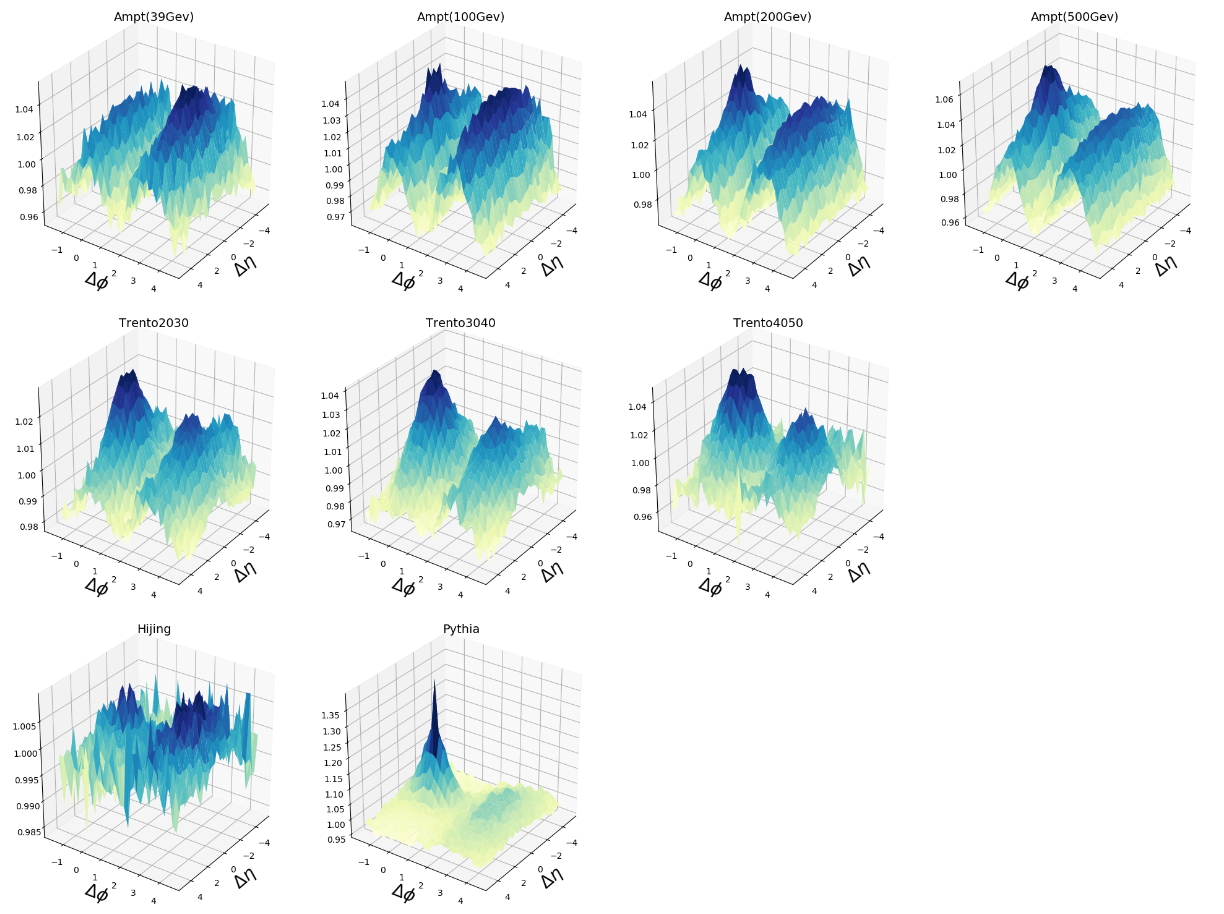
\includegraphics[width=140mm]{sample}
\caption{\label{fig:sample}%
各模型得到的二粒子关联图像示意图,各图均是在大量事件平均的基础上得到的,前两行是流事件模型,第三行是非流事件模型}
\end{figure}
\subsubsection{流与非流事件的主成分分析}
我们首先采用主成分分析的方法来对流与非流事件进行分类,需要提及的一点是,我们在用主成分分析是所用到的二粒子关联函数
并非式~\ref{eq:5} 中的$C(\Delta\phi,\Delta\eta)$,而是其中的$S(\Delta\phi,\Delta\eta)$,如图~\ref{fig:pcasample} 所示。在这里,我们使用Ampt(39Gev)、
Trento2030、Hijing三个模型进行主成分分析,得到的结果如图~\ref{fig:pcaresults} 所示。其中左图表示的是使用主成分分析找出的各个主成分对应的本征值大小,本征值越大
表明,此主成分对应的特征向量越能表示数据的性质。从左图可以看出,有两个特征值特别大,因此,这两个特征值对应的特征向量即可表示数据的大部分特征,因此做出数据在这两个特征向量
构成的平面上的分布图,如右图所示,可以发现在这两个特征向量下,数据被很好的区分开。而这两个特征向量如图~\ref{fig:tzxl} 所示,可以发现,这两个特征向量均刻画了前面提及的
流事件的双脊效应,因此,在一定程度上主成分分析找到了流与非流事件的区别。我们可以考虑将这两个特征向量进行线性组合得到流与非流事件的区别,如图~\ref{fig:qb} 所示,
黑线即是这两个特征向量进行线性组合构造的流与非流事件的分界线,黑线右上方认为是流事件,左下方认为是非流事件。
在此分界线下,用Ampt(200Gev)的数据进行测试,结果如图~\ref{fig:cs} 所示,可以看出,测试结果符合我们的预期。但是必须指出的是,此黑线的划定有很大的自由度,因此很难精确
的区分流与非流的混合事件。同时,从数据的分布可以看出,此结果具有很强的模型依赖性,而这对我们寻找流和非流的本质区别是有害的,因此我们需要其他的方法来精确的确定流与非流的本质区别,下面
我们将用神经网络进行尝试。
\begin{figure}[htbp]
\centering
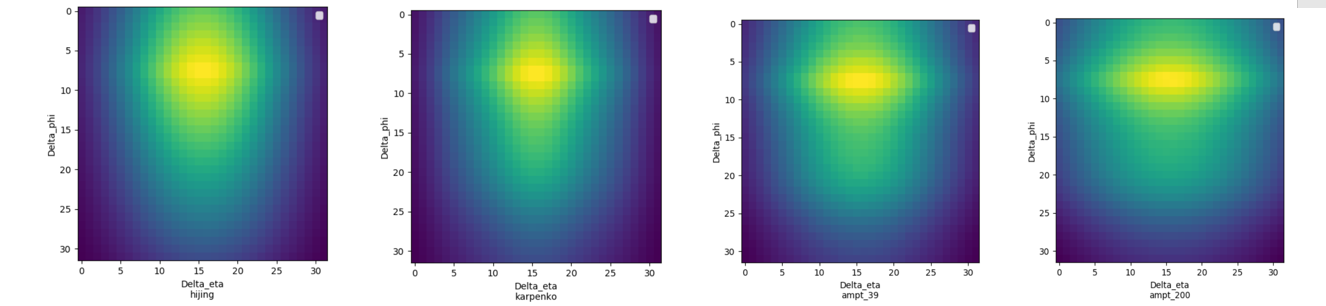
\includegraphics[width=140mm]{pcasample}
\caption{\label{fig:pcasample}%
Hijing,Trento2030\footnote{图中表示为Karpenko},Ampt(39Gev),Ampt(200Gev)在大量事件平均下$S(\Delta\phi,\Delta\eta)$的示例图}
\end{figure}
\begin{figure}[htbp]
\centering
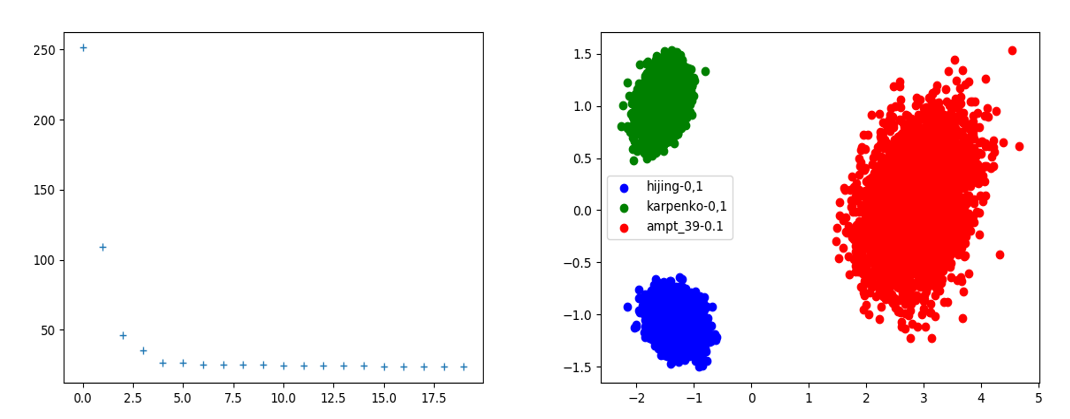
\includegraphics[width=140mm]{pcaresults}
\caption{\label{fig:pcaresults}%
对Hijing,Trento2030\footnote{图中表示为Karpenko},Ampt(39Gev)进行主成分分析得到的结果图,左图是各个特征向量对应的特征值大小,右图为输入数据在第一个和第二个
特征向量组成的平面上的分布}
\end{figure}
\begin{figure}[htbp]
\centering
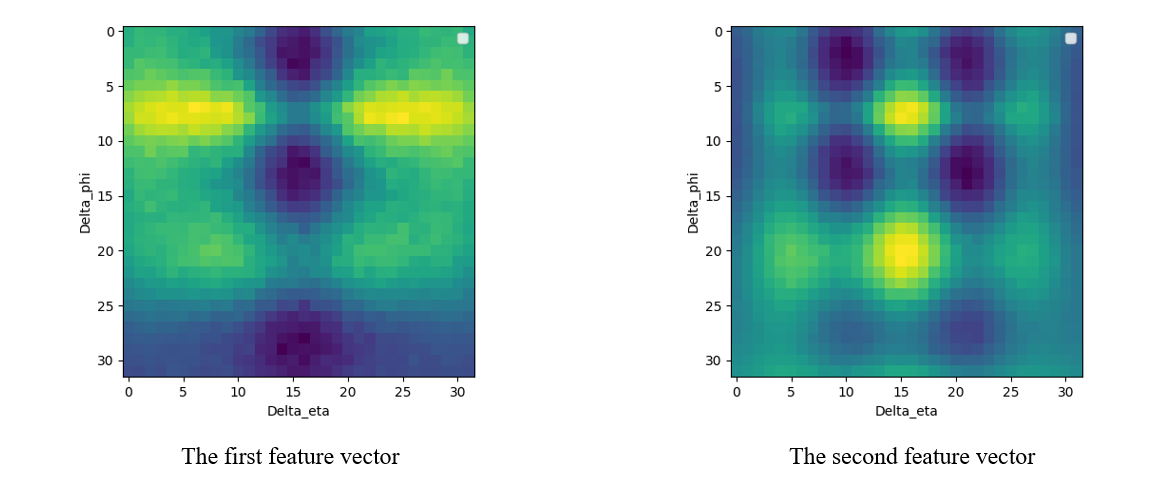
\includegraphics[width=140mm]{tzxl}
\caption{\label{fig:tzxl}%
对Hijing,Trento2030,Ampt(39Gev)进行主成分分析得到的
第一第二个特征向量,左边为第一个,右边为第二个,横坐标为$\Delta\eta$,0-32表示的是$\Delta\eta\in(-5,5)$
,纵坐标为$\Delta\phi$,0-32表示的是$\Delta\phi\in[-0.5\pi,1.5\pi)$}
\end{figure}
\begin{figure}[htbp]
\centering
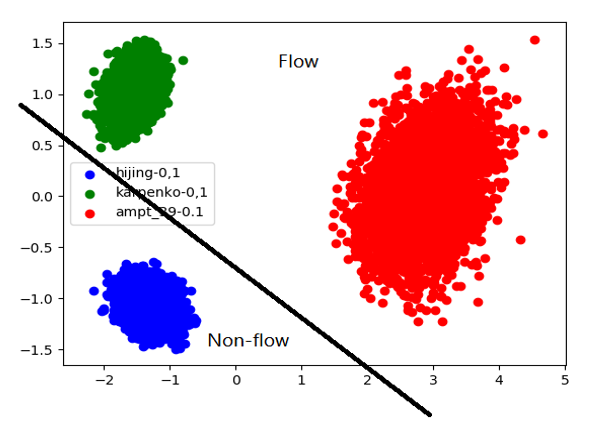
\includegraphics[width=140mm]{qb}
\caption{\label{fig:qb}%
假定的流与非流事件的分界线,即图中黑线所示}
\end{figure}
\begin{figure}[htbp]
\centering
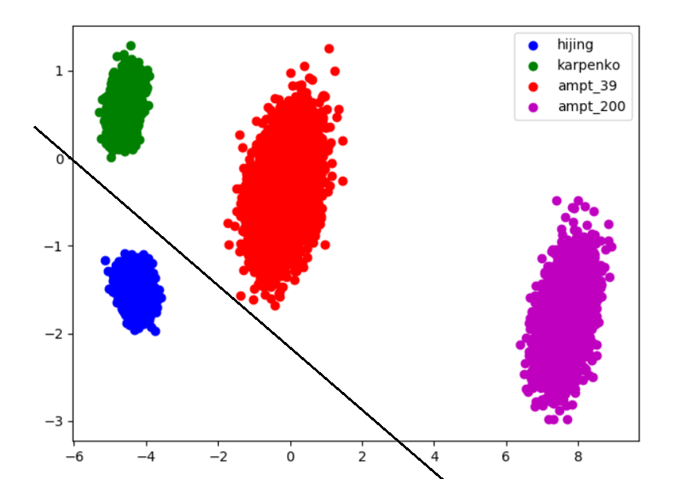
\includegraphics[width=140mm]{cs}
\caption{\label{fig:cs}%
用Ampt(200Gev)的数据测试假定的流与非流事件的分界线,即图中黑线所示}
\end{figure}
\subsubsection{流与非流事件的神经网络分类分类}
实验中所用到的卷积神经网络结构如图~\ref{fig:sjwl} 所示,同时所用到的二粒子关联函数
为式~\ref{eq:5} 中的$C(\Delta\phi,\Delta\eta)$,其样式如图~\ref{fig:sample} 所示。我们将流事件标记为(1,0),将非流事件标记为(0,1),然后
让神经网络学习从输入数据到标签的映射,最终训练好的网络将能够实现对流与非流事件的分类。
我们在输入层输入数据,然后两次经过卷积核为3*3的卷积层和最大池池化层,再展开为向量,经过两次全连接后,通过
输出层输出。在整个过程中,除输出层所用激活函数为Softmax外,其余均为Relu。所用损失函数为交叉熵损失函数。\par
训练网络时,首先我们选择仅用一个流模型与非流模型的100个事件平均后的数据各5000组作为训练集,之后用所有的模型下的100个
事件平均后的各10000组数据作为测试集来测试网络的结果,测试的准确度是指,网络输出正确标签的组数占总组数的百分比。
得到的结果如表~\ref{table:1} 所示,可以看出,仅用一种流与非流模型作为训练集的话,总会有个别模型的结果表现十分差,这表明我们的输入数据不足,使得网络
并未学到流与非流之间本质区别。\par
之后将所有流与非流模型的数据均作为训练集,
得到的结果如表~\ref{table:2} 所示,可以看出,在我们用所有的流与非流模型作为训练后,网络可以在测试集上的表现十分好,
同时我们研究了在不同事件平均下网络的表现结果,即对涨落压制在程度强弱下,网络的表现结果,可以看出,在1000、100、50个事件平均下,网络的表现都十分
良好,这表明,涨落在对于网络的分辨本领影响并不是十分巨大,只要在一定的事件数平均下,对涨落造成了一定程度上的抑制,网络
就可以得到一个比较好的表现结果。
\begin{figure}[htbp]
\centering
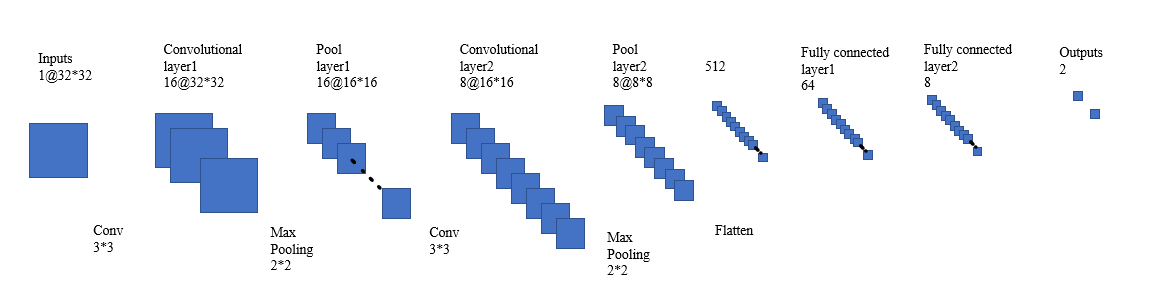
\includegraphics[width=140mm]{sjwl}
\caption{\label{fig:sjwl}%
鉴别流与非流所用到的卷积神经网络结构图}
\end{figure}
\begin{table}[htbp]
\caption{\label{tab:table1}%
在不同训练集训练下,测试集上网络的表现行为,所用到的所有数据都是在100个事件平均下的结果}
\begin{ruledtabular}
\begin{tabular}{lllll}
测试集 & 准确度1\footnote{此结果使用的训练集为Ampt(39Gev)、Ampt(200Gev)、Hijing}
 &准确度2\footnote{此结果使用的训练集为Ampt(39Gev)、Ampt(100Gev)、Ampt(200Gev)、Ampt(500Gev)、Pythia}
 &准确度3\footnote{此结果使用的训练集为Trento2030、Trento3040、Hijing}
 &准确度4\footnote{此结果使用的训练集为Trento2030、Pythia} \\
\colrule
Ampt(39Gev)&99.95\%&98.88\%&100\%&0\% \\
Ampt(100Gev)&98.77\%&100\% &100\%&80.08\%\\
Ampt(200Gev)&97.75\%&100\% &100\%&100\%\\
Ampt(500Gev)&99.57\%&100\% &99.57\%&100\%\\
Trento2030&4.99\%&100\% &99.59\%&100\%\\
Trento3040&58.22\%&100\% &100\%&100\%\\
Trento4050&97.89\%&100\% &100\%&99.78\%\\
Hijing&99.98\%&0\% &99.11\%&0\%\\
Pythia&0\%&100\% &0\%&100\%\\
\end{tabular}
\end{ruledtabular}
\end{table}
\begin{table}[htbp]
\caption{\label{tab:table2}%
在相同训练集训练,在不同数目事件平均下,测试集上网络的表现行为\footnote{所用到的训练集数据均为Ampt(39Gev)、Ampt(500Gev)、Trento3040、Hijing、Pythia}}
\begin{ruledtabular}
\begin{tabular}{llll}
测试集 & 准确度1\footnote{此结果是在1000个事件平均下的结果}
    &准确度2\footnote{此结果是在100个事件平均下的结果}
    &准确度3\footnote{此结果是在50个事件平均下的结果}\\
\colrule
Ampt(39Gev)&100\%&100\%&99.93\%\\
Ampt(100Gev)&100\%&100\% &91.82\%\\
Ampt(200Gev)&100\%&100\% &99.65\%\\
Ampt(500Gev)&100\%&100\% &100\%\\
Trento2030&99.97\%&99.99\% &99.97\%\\
Trento3040&100\%&100\% &100\%\\
Trento4050&100\%&100\% &100\%\\
Hijing&99.99\%&99.96\% &100\%\\
Pythia&100\%&100\% &100\%\\
\end{tabular}
\end{ruledtabular}
\end{table}
\subsection{利用人工神经网络拟合相对论性重离子碰撞演化}
\subsubsection{问题定义,数据处理及网络结构}
\begin{enumerate}
    \item 问题提出与定义:\par
    利用TRENTO+VISHNU的联合模型,可以很好的描述相对论性重离子碰撞的演化过程。因而,一旦确定了TRENTO与VISHNU的参数,在多事件平均压制涨落的基础上,可以近似确定产生的末态粒子分布,既而确定末态粒子的观测量。\par
因此,利用TRENTO+VISHNU模型,确定演化参数与末态观测量之间的关系,进而应用于真实的实验数据中,便可以获得对应于真实数据的演化参数。\par
通过不同的参数选择,TRENTO可以给出近似各种模型的初态分布,通过TRENTO参数的确定,我们或许可以选择最为接近实际的初态模型;而通过VISHNU参数的确定,我们可以直接确定QGP自身的宏观物理性质。\par
    \item 数据选择及处理:\par
    数据的选取分为两个方面,一方面是模型参数,另一方面是观测量:
    \begin{enumerate}
        \item 对于初态模型,我们将TRENTO所用到的所有参数都作为输入,包括有总规范化因子$\mathrm{N}$、约化密度参数$p$、权重因子抽样符合的gamma分布参数$k$以及粒子分布与能量密度转换参数:核子有效宽度$\omega$;
        \item 对于流体演化混合模型,我们所需要的参数有:流体的粘滞系数,分别为剪切粘滞系数$\eta/s$,体粘滞系数$\zeta/s$,以及转变温度$T_{switch}$。在演化过程中,粘滞系数事实上是温度的函数,在我们使用的模型中,
        认为在转变温度之上,强子气体的$\eta/s$是一个常数,而且是对于各种参数条件取值都相等,因此我们无法拟合;而在转变温度之下,QGP的$\eta/s$随着温度的上升呈线性变化,可以用最小值和斜率来描述;同时,对于$\zeta/s$,
        模型将通过调制整体归一化系数完成控制。
        \item 对于末态粒子观测量,在相对论性重离子碰撞中,粒子的产量$dN/d\eta$以及集体流系数$v_n$,是描述碰撞事件末态的重要指标,因此我们选择使用这些观测量来进行系数的拟合,同时,将所选择的观测量按照中心度进行离散化。\par
    \end{enumerate}
    综上,数据的选取如表\ref{tab:bnn}所示,我们取末态观测量为输入,而取模型参数为输出,进行直接拟合。
    \item 神经网络结构的选取:\par
    由于相对论性重离子碰撞的模拟十分消耗计算资源,而为了压低涨落,所需要的模拟事件数目更多,因此,只拥有250组数据供训练,50+1组数据供测试。所以,在本课题中采用贝叶斯神经网络进行拟合。我们对各个参数独立拟合,各网络的结构如图\ref{fig:bnn}。    
\end{enumerate}
\begin{table}[htbp]
\caption{利用人工神经网络拟合重离子碰撞演化数据选取\label{tab:bnn}}
\begin{ruledtabular}
\begin{tabular}{p{4cm}p{4cm}p{4cm}p{4cm}}
参数&类别&描述&输入/输出\\
\colrule
初态总规范化因子$\mathrm{N}$&初态TRENTO参数&描述了初态的总规模大小&输出\\
约化厚度参数$p$&初态TRENTO参数&两核子厚度耦合参数&输出\\
gamma分布参数$k$&初态TRENTO参数&控制涨落大小&输出\\
有效宽度$\omega$&初态TRENTO参数&描述粒子于能量密度的转换&输出\\
\colrule
QGP剪切粘滞系数最小值$\eta/s_{min}$&QGP演化模型VISHNU参数&描述QGP剪切粘滞系数与温度的关系&输出\\
QGP剪切粘滞系数斜率$\eta/s_{slope}$&QGP演化模型VISHNU参数&描述QGP剪切粘滞系数与温度的关系&输出\\
QGP体粘滞系数规范化因子$\zeta/s_{norm}$&QGP演化模型VISHNU参数&QGP体粘滞系数在演化过程中的控制&输出\\
QGP/强子化转变温度$T_{switch}$&QGP演化模型VISHNU参数&QGP/强子气体相变的开始&输出\\
\colrule
$K^{\pm},\pi^{\pm},p\bar{p}$的产量$dN/dy$&末态粒子观测量&按中心度(\%)划分:0−5,5−10,10−20,……,60−70,70−80&输入\\
$K^{\pm},\pi^{\pm},p\bar{p}$的横向动量平均值$\langle p_{T}\rangle$&末态粒子观测量&按中心度(\%)划分:0−5,5−10,10−20,……,60−70,70−80&输入\\
总二阶流$v_2$&末态粒子观测量&按中心度(\%)划分:0−5,5−10,10−20,……,70−80&输入\\
总三阶流$v_3$&末态粒子观测量&按中心度(\%)划分:0−5,5−10,10−20,……,40-50&输入\\
总四阶流$v_4$&末态粒子观测量&按中心度(\%)划分:0−5,5−10,10−20,……,40-50&输入\\
\end{tabular}
\end{ruledtabular}
\end{table}
\begin{figure}[htbp]
\centering
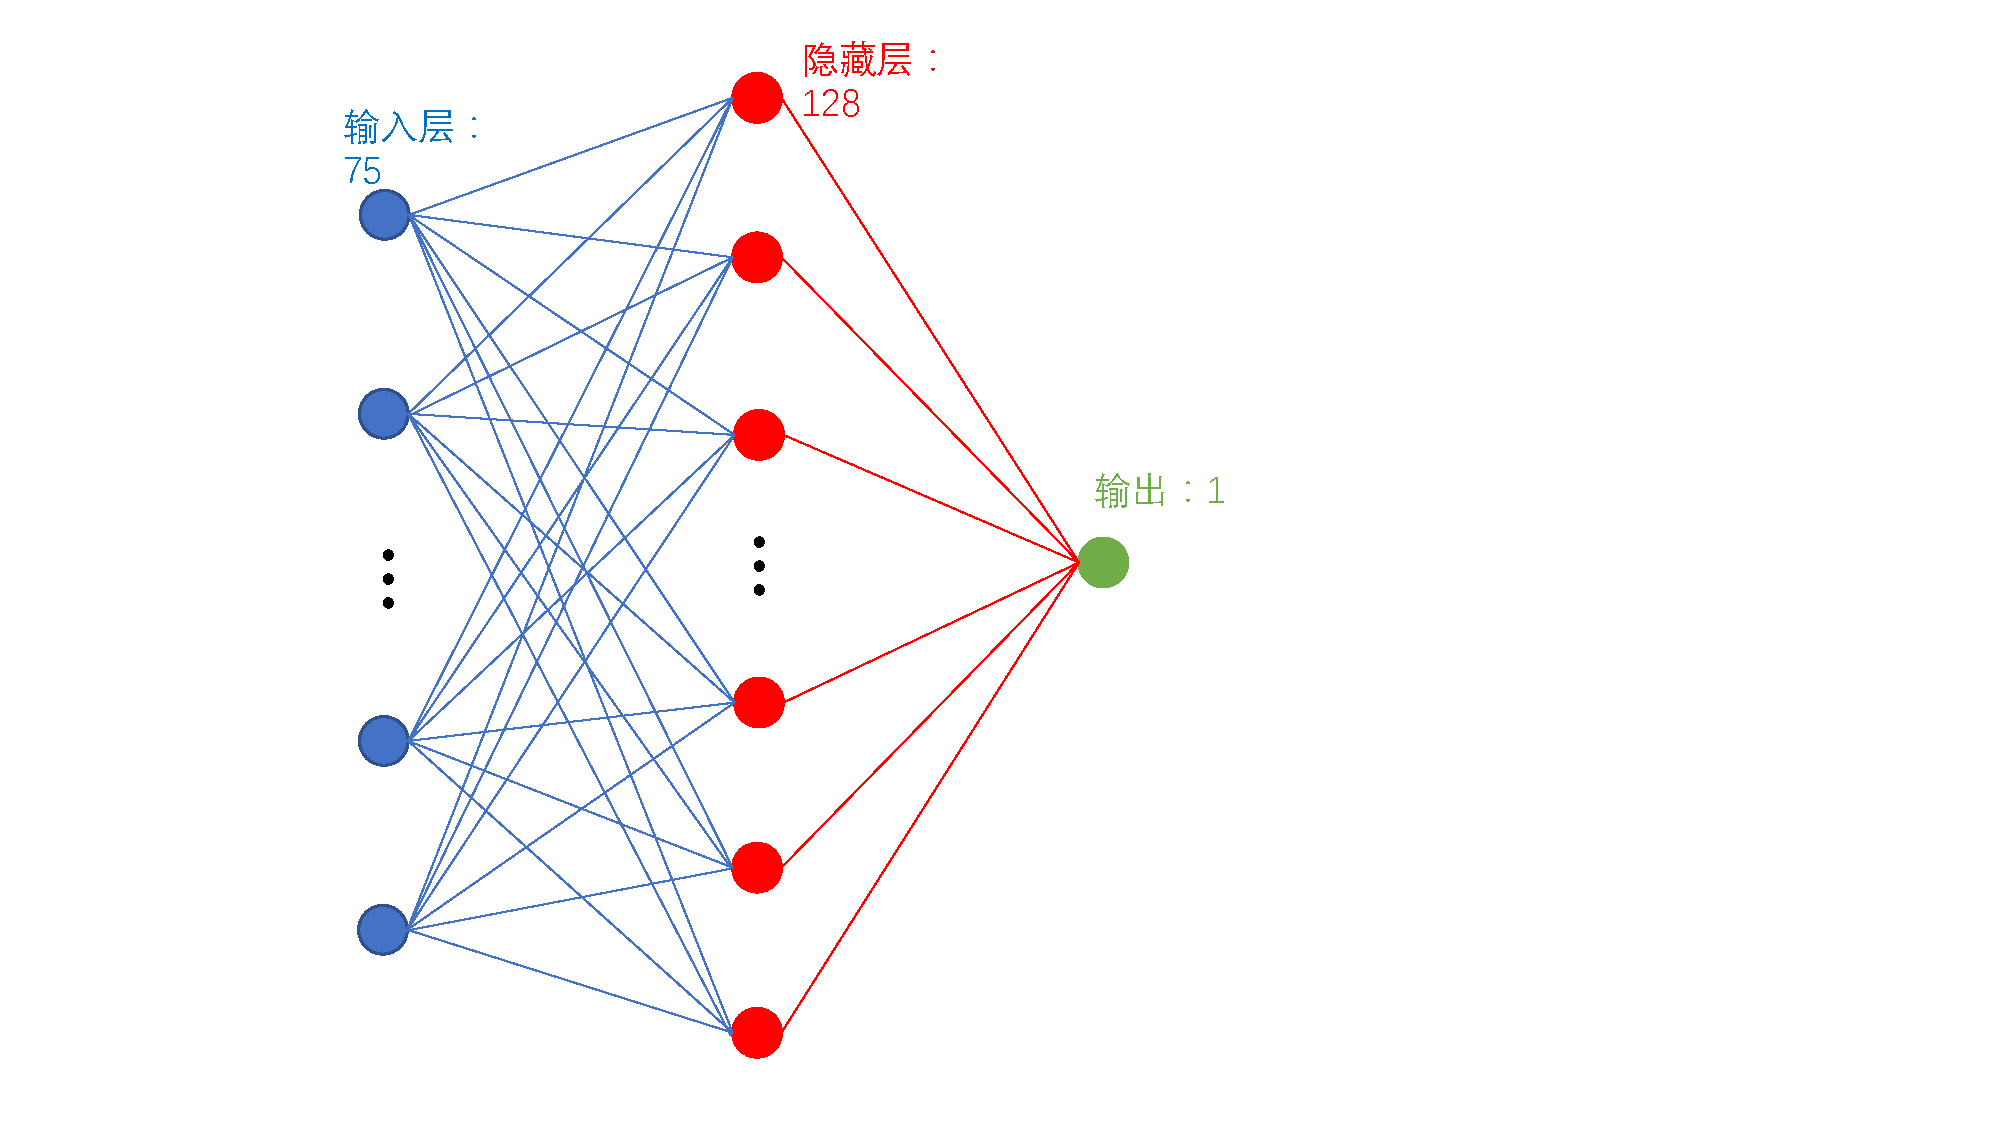
\includegraphics[width=0.5\textwidth]{bnn}
\caption{贝叶斯神经网络结构图\label{fig:bnn}}%
\end{figure}
\subsubsection{结果与分析}
经过训练后,神经网络在测试集上的表现如图\ref{fig:bnnoutput}所示:\par
\begin{figure}[htbp]
\centering
\subfloat[$\zeta/s_{norm}$]{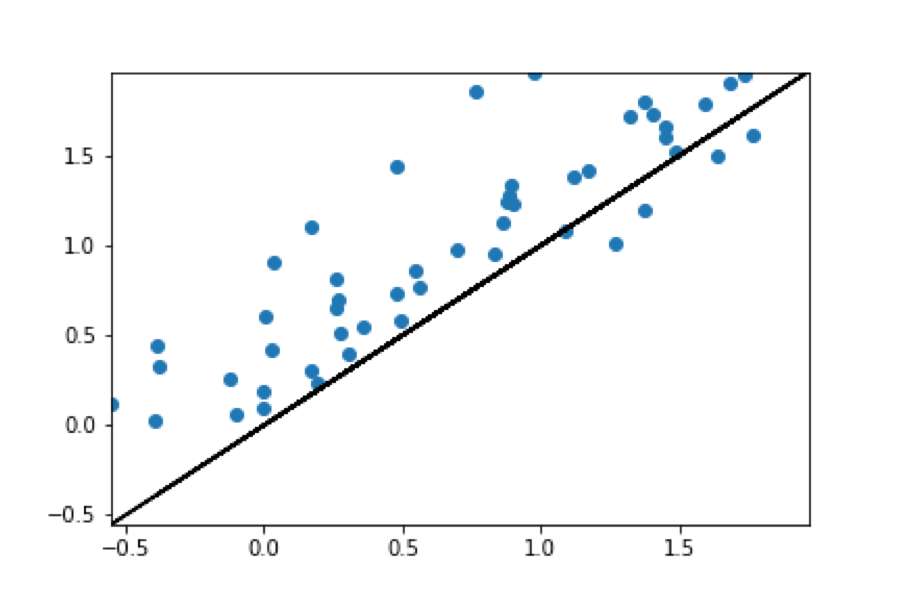
\includegraphics[width = 0.2\textwidth]{fig_1.png}}
\subfloat[$\eta/s_{slope}$]{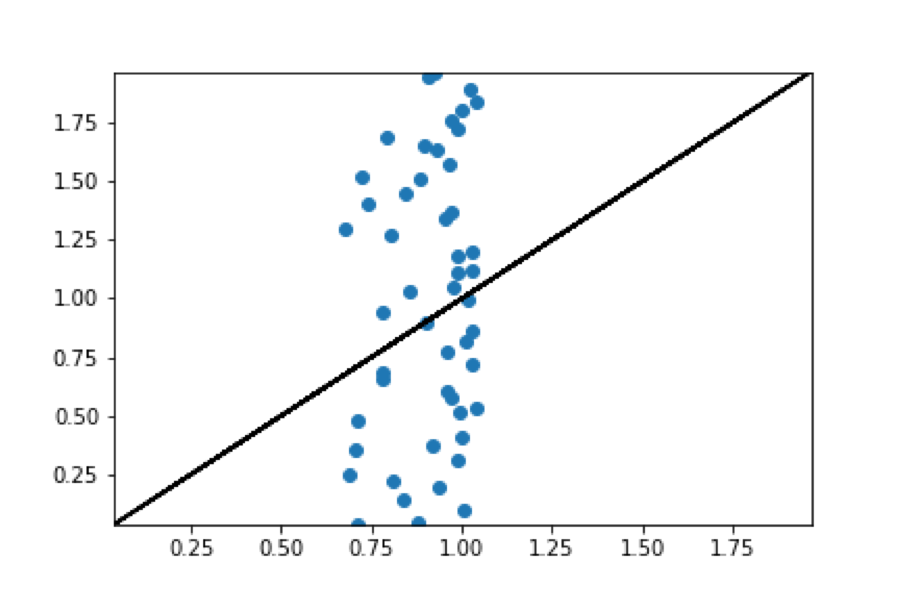
\includegraphics[width = 0.2\textwidth]{fig_2.png}}
\subfloat[$T_{switch}$]{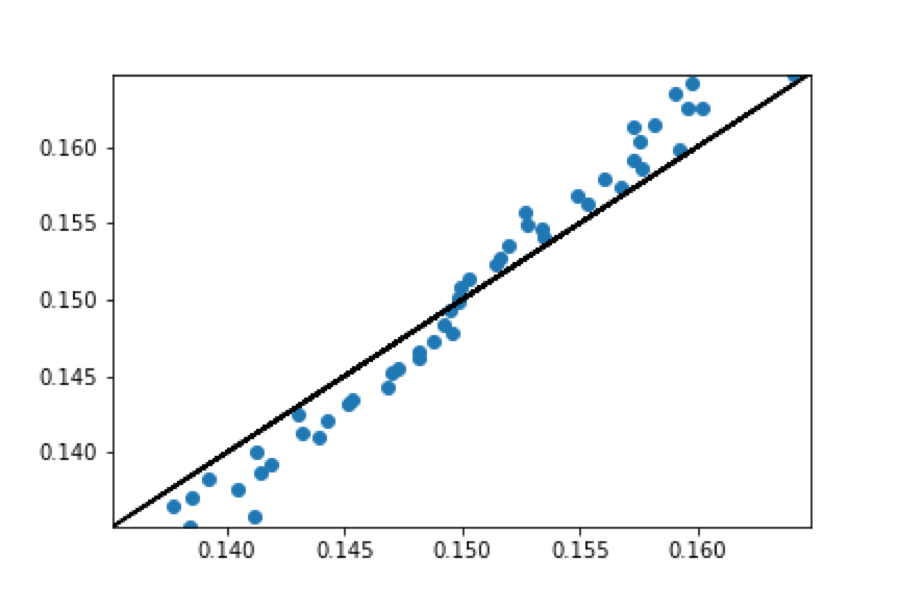
\includegraphics[width = 0.2\textwidth]{fig_3.png}}
\subfloat[$\eta/s_{min}$]{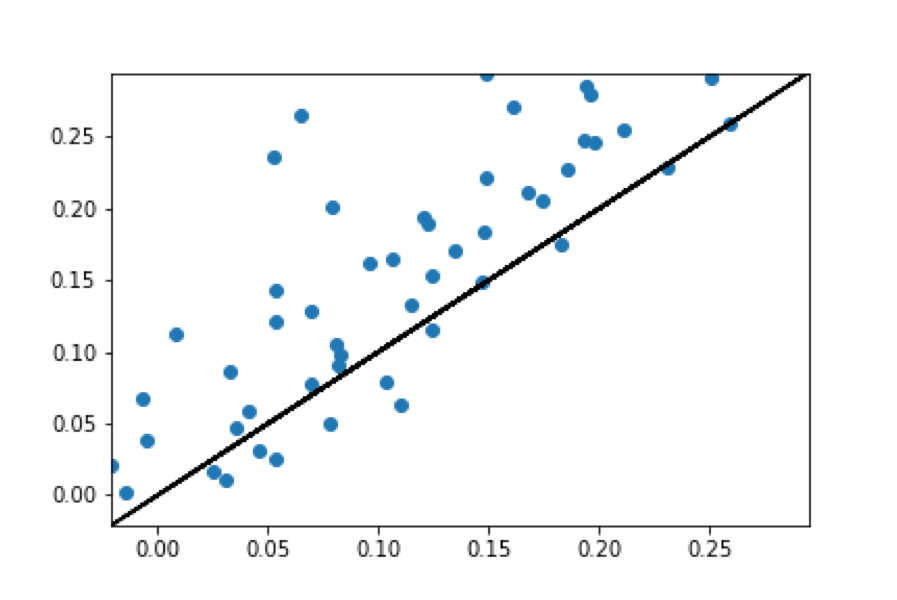
\includegraphics[width = 0.2\textwidth]{fig_4.png}}\\
\subfloat[$\mathrm{N}$]{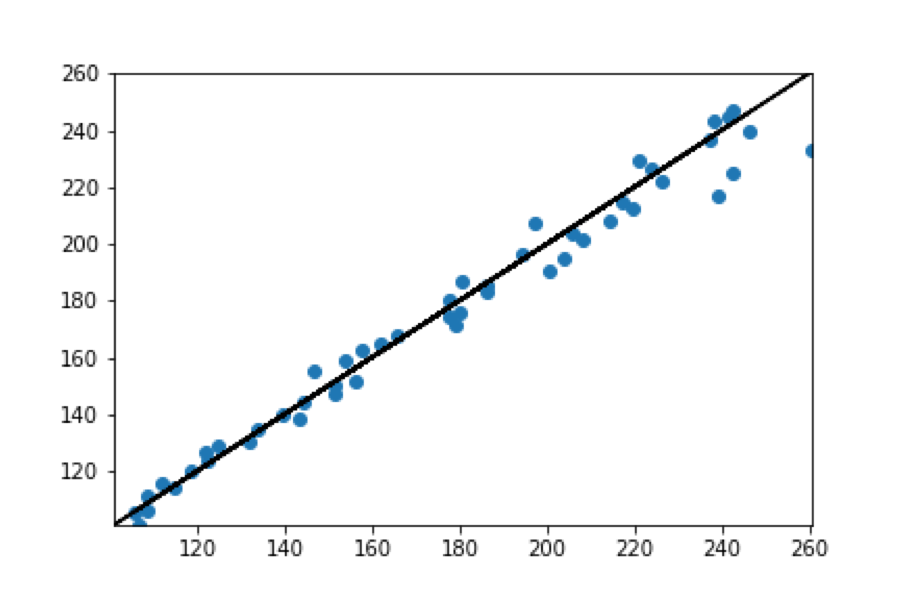
\includegraphics[width = 0.2\textwidth]{fig_5.png}}
\subfloat[$p$]{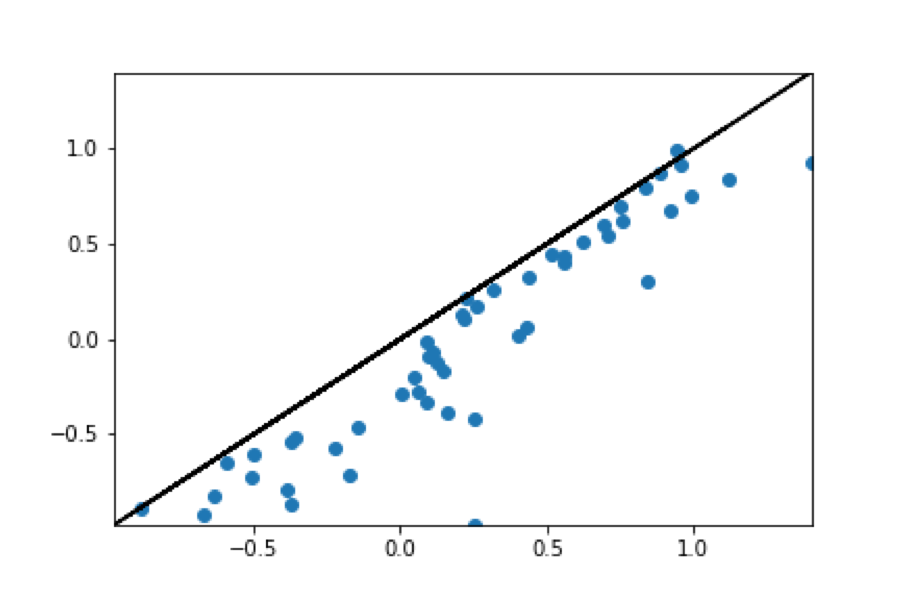
\includegraphics[width = 0.2\textwidth]{fig_6.png}}
\subfloat[$w$]{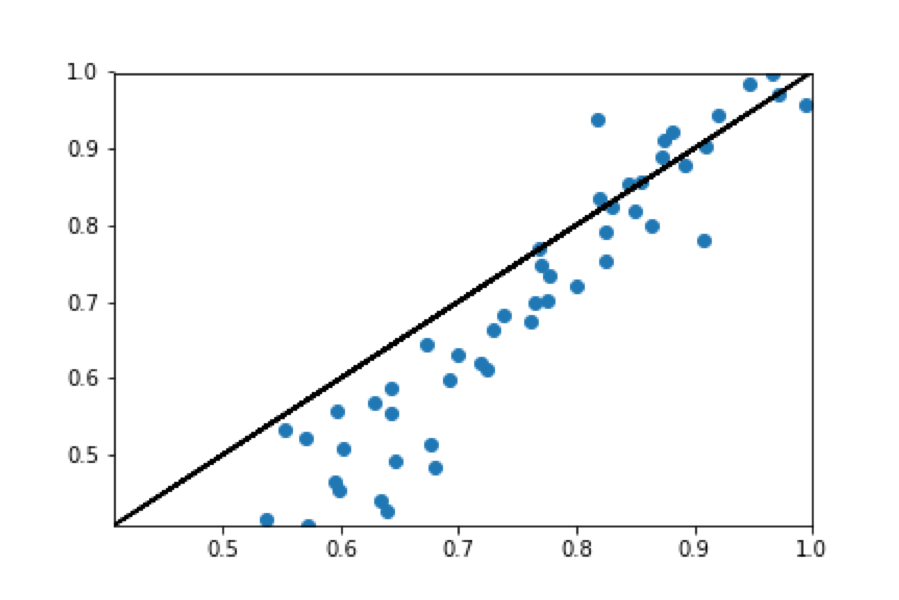
\includegraphics[width = 0.2\textwidth]{fig_7.png}}
\subfloat[$k$]{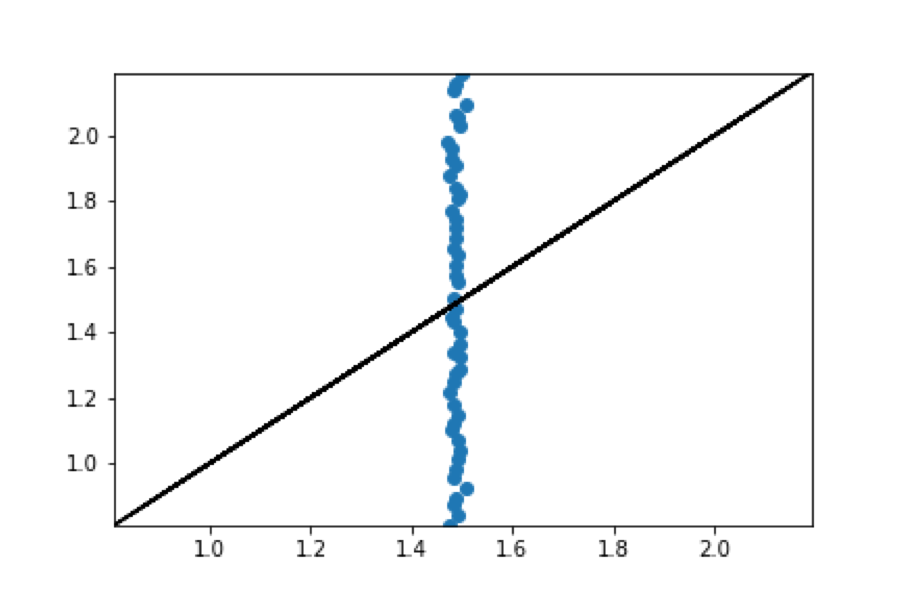
\includegraphics[width = 0.2\textwidth]{fig_8.png}}\\
\caption{贝叶斯神经网络在测试集上的表现\label{fig:bnnoutput}}
\end{figure}
继而,将其应用到ALICE的实验数据中,可以获得拟合参数如表\ref{tab:ALICEdata}:\par
\begin{table}[htbp]
\caption{贝叶斯神经网络在实验数据上的表现\label{tab:ALICEdata}}
\begin{ruledtabular}
\begin{tabular}{ccccccccc}
参数&$\mathrm{N}$&$p$&$w$&$k$&$\eta/s_{slope}$&$\eta/s_{min}$&$\zeta/s_{norm}$&$T_{switch}$\\
\colrule
神经网络给出拟合&120。5&0&1.47&0.47&0.86&0.10&1.29&0.153\\
最佳拟合&120&0&1.5&0.43&0.85&0.08&1.25&0.148
\end{tabular}
\end{ruledtabular}
\end{table}
可以看出,神经网络在部分参数上可以给出较好的拟合精度,而在一些参数上预测效果则不够理想。当然,由于存在观测量对于参数敏感性的问题,我们还是应该计算观测量并与实验值对比,才能完成更好的判断。\par
由于相对论性重离子碰撞的模拟需要大量的计算资源,我们只选取集体流系数进行计算,如图\ref{fig:alice}展示了集体流系数的计算结果。\par
\begin{figure}[htbp]
\centering
\subfloat[针对ALICE实验结果拟合参数的相对误差]{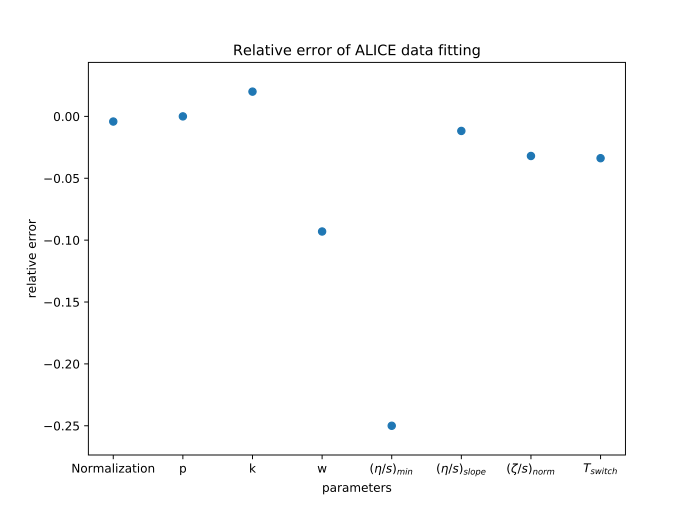
\includegraphics[width=0.4\textwidth]{alice.png}}
\subfloat[利用拟合参数计算的集体流(1200events),实线是网络预测结果,点是验证集中数据]{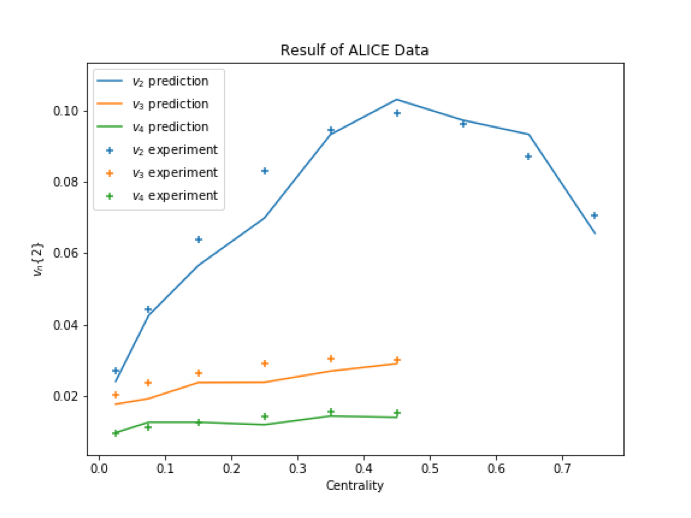
\includegraphics[width=0.4\textwidth]{alice_v2.png}}
\caption{针对ALICE实验结果的集体流计算\label{fig:alice}}%
\end{figure}
此外,我们同时在验证集中随机选取了两组,同样计算了集体流系数,结果如图\ref{fig:valid}:\par
\begin{figure}[htbp]
    \centering
    \subfloat[验证集数据一]{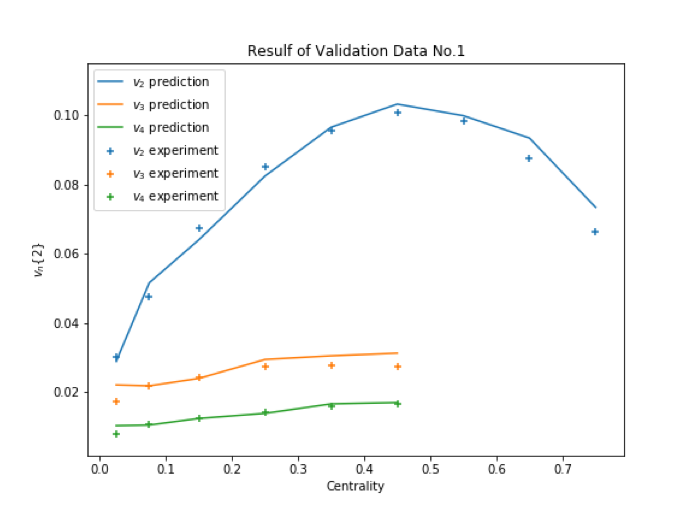
\includegraphics[width=0.4\textwidth]{v_1.png}}
    \subfloat[验证集数据二]{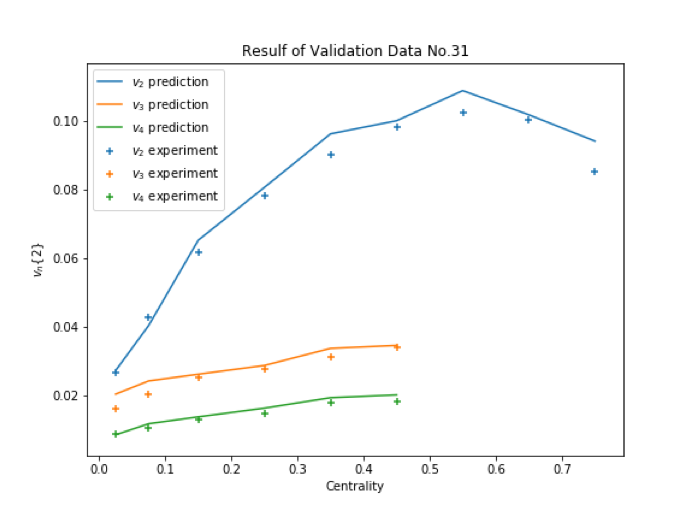
\includegraphics[width=0.4\textwidth]{v_2.png}}
    \caption{验证集数据的集体流计算(990events),实线是网络预测结果,点是验证集中数据\label{fig:valid}}%
    \end{figure}
从以上结果中可以看出,神经网络预测的参数,可以对集体流给出一个较好的拟合,由于算力的限制,我们模拟的碰撞事件数不够,这可能是拟合差距的主要来源。
\subsection{利用贝叶斯展开研究集体流长程解关联现象}
\subsubsection{问题定义,数据产生与处理}
\begin{enumerate}
    \item 问题提出与定义:\par
    在相对论性重离子碰撞领域的实验数据处理中,一个重要的问题是如何减少探测器的影响。探测器不仅仅会带来效率上的损失,有时往往还伴随着随机噪声,使本来狭窄的信号分布展宽。而在对集体流效应的研究中,压低非流信号的影响也十分重要。
    \par
    处理积分流时(在$\eta$方向进行积分,而前向后向的分布应当是完全相关的)贝叶斯展开有着很好的表现,可以同时完成上述功能。\par
    但是,如果要利用贝叶斯展开研究集体流长程解关联行为,问题就会变得非常复杂。
    \begin{enumerate}
        \item 集体流的解关联行为不仅表现在集体流矢量的幅度上,也表现在集体流矢量的形状和相位上。因此,若要描述整个体系,需要一个高维的相空间。而高维的相空间所消耗的计算资源将十分巨大,行为也会更加混乱。
        \item 事实上,解关联这一行为的强度并不高,因此在整个相空间中,解关联行为是非常局域化的。局域化带来了一些便利,例如可以减少相空间内区域的个数;但是,局域化的分布意味着在相空间中存在着概率较小点,对于这些点的处理,迭代次数过多会带来巨大涨落,迭代次数较少收敛效果可能较差。
    \end{enumerate}
    因此,在应用到实验数据之前,需要仔细地检验贝叶斯展开这一工具的效果,并通过检验效果考虑是否应用于实验数据。
    \item 解关联模型的建立:\par
    我们采取一个简单的解关联模型来完成这一检验。\par
    \begin{enumerate}
        \item 虽然,不同$\eta$区间内,集体流矢量需要相角和幅度共同描述。但是,首先我们关心的是两者的关联程度,因此只有相对相位有意义,相空间可被减少为3维;其次,解关联行为的强度不高,两者的幅度应该较为接近,因此可以采用幅度的算术平均值
        和幅度差来衡量,可以减少相空间内一个维度的总大小;最后,不妨仅取相对相位与幅度差的绝对值,可以将相空间的体积再次缩减,减少消耗的计算资源。
        \item 我们采取如下的解关联模型实现:\par
        实验上对于解关联的测定,常常是通过前向后向$\eta$绝对值相同区间来实现,根据式\ref{eq:decorr},对于$\eta$,$-\eta$,可以认为其解关联效应完全相反。
        因此,可以首先产生两者正关联的部分$\vec{v}_0$,再产生反关联的$\vec{d}$,最后分别添加一随机向量$\vec{s}_\pm$,模拟展宽效应。
        \begin{equation}
            \begin{aligned}
                \vec{v}_+&=\vec{v}_0+\vec{d}+\vec{s}_+\\
                \vec{v}_-&=\vec{v}_0-\vec{d}+\vec{s}_-
            \end{aligned}
        \end{equation}
        \item 即使我们的模型非常简单,我们仍希望这一模型能够尽量符合实验上的观测,因而仔细设计了数据的产生:\par
        在真实的相对论性重离子碰撞实验中,我们需要处理的事件数目十分巨大,因此,可以利用中心极限定理。对于上述矢量,均可以处理成二维高斯分布,相应的,模长应该符合贝塞尔高斯分布。举例来说,集体流矢量幅度的分布应该满足贝塞尔高斯分布,形式如下:\par
        \begin{equation}
            p\left(v_{n}^{\mathrm{obs}} | v_{n}\right) \approx \frac{1}{2 \pi \delta_{n}^{2}} v_{n}^{\mathrm{obs}} e^{-\frac{\left(v_{n}^{\mathrm{obs}}\right)^{2}+v_{n}^{2}}{2 \delta_{n}^{2}}} I_{0}\left(\frac{v_{n}^{\mathrm{obs}} v_{n}}{\delta_{n}^{2}}\right)
        \end{equation}
        \par
        其中,$v_{n}^{\mathrm{obs}}$代表观测量,其均值为$v_n$,宽度为$\delta_n$。
        在我们的解关联模型中,所有的矢量都来自于二维高斯分布(或直接来自于贝塞尔高斯分布)。同时,定义比值:\par
        \begin{equation}
            F=\frac{\langle v_1v_2^*\rangle}{\langle|v_0|^2\rangle}
        \end{equation}
        使之与实验上的解关联效应相仿。
        \item 在实施贝叶斯展开的时候,需要预先选择两个合理的先验分布,其一是产生迁移矩阵(条件概率)的分布,其二是进行迭代的分布。\par
        迁移矩阵的分布要求不能过宽,否则需要大量的抽样以压低涨落,亦不能过窄,因为从数值上看,
        $A_{ij}=0$,既可能是条件概率为零,也可能是先验分布为零,两者无法区分,故而这一先验分布应该涵盖目标分布所有可能的相空间范围,同时尽可能狭窄。\par
        进行迭代的先验分布,从收敛的速度上考虑,我们要求其尽可能接近真实的分布,并且包含之。\par
        因此,一个合理的选择是展宽后的分布,因为根据展宽效应,其涵盖了可能的真实分布,并且,我们无法进行进一步的限制。
    \end{enumerate}
    \item 数据处理:
    \begin{enumerate}
        \item 为了获得与实验上相吻合的数据,我们选取关联部分来自于均值为$0.08$,宽度为$0.035/\sqrt{2}$的贝塞尔高斯分布。而对于反关联部分,我们采用均值为$0.02$,宽度为$0.01$的贝塞尔高斯分布,对于两部分间的夹角,在$(0,2\pi)$间均匀选取。最后,为前后向分别加上展宽效应:在两垂直方向上分别加入$\mu=0,\sigma=0.025$的高斯分布。
        \item 为了减少计算量,一个有用的方式是进行不均匀区间划分,我们数据的划分如表\ref{tab:bu1}所示。
    \end{enumerate}
    \begin{table}[htbp]
    \caption{\label{tab:bu1}}
    \begin{ruledtabular}
    \begin{tabular}{c|c|c}
    维度&划分方式&区间数\\
    \colrule
    $(v_++v_-)/2$&0-0.02: 宽度0.01;
    0.02-0.2: 宽度0.006;
    0.2-0.3: 宽度0.01;
    &42\\
    $|v_+-v_-|/2$&0-0.03: 宽度0.005;
    0.03-0.07: 宽度0.01;&10\\
    $|\Delta\Psi|$&0-$3\pi/7$: 宽度$\pi/14$;
    $3\pi/7$-$\pi$: 宽度$\pi/7$;&10    
    \end{tabular}
    \end{ruledtabular}
    \end{table}
\end{enumerate}
\subsubsection{结果与分析}
为了进行仔细的检验,我们选取了一维边缘分布,二维边缘分布,三维边缘分布分别进行贝叶斯展开。
\begin{enumerate}
    \item 一维边缘分布:\par
    一维边缘分布的结果如图\ref{fig:bu1d}所示。\par
    \begin{figure}[htbp]
    \centering
    \subfloat[$(v_++v_-)/2$]{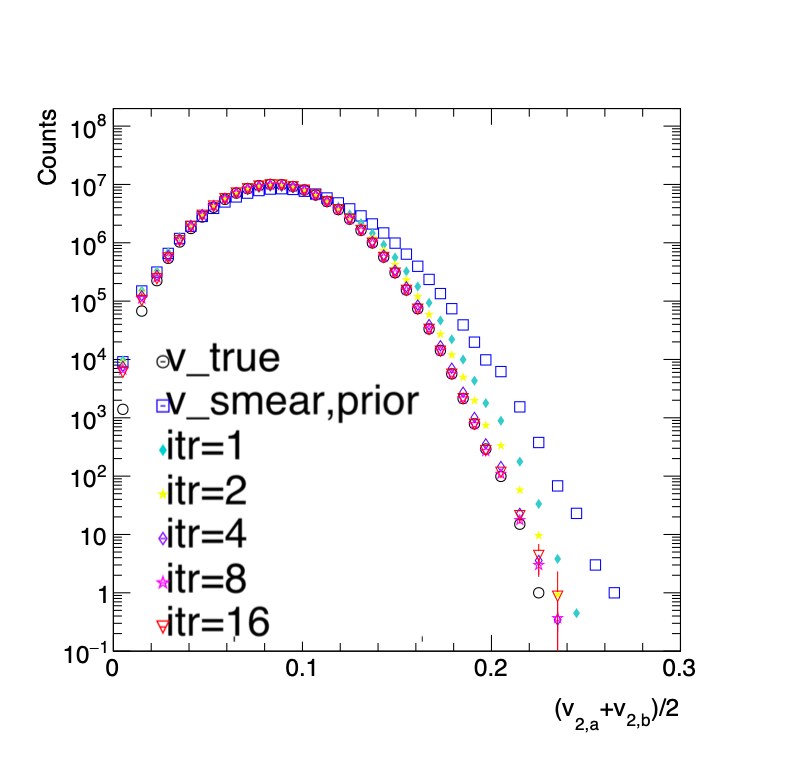
\includegraphics[width=0.3\textwidth]{1d_vp.png}}
    \subfloat[$|v_+-v_-|/2$]{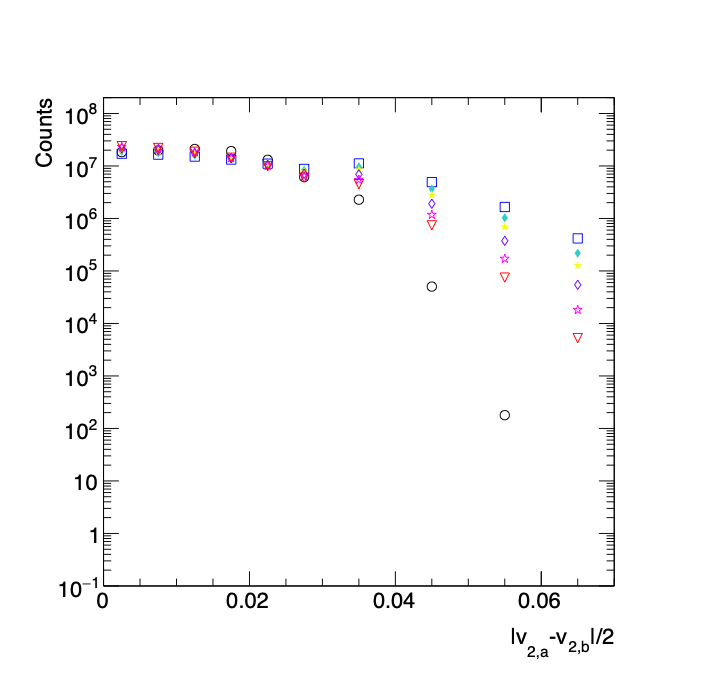
\includegraphics[width=0.3\textwidth]{1d_vm.png}}
    \subfloat[$|\Delta\Psi|$]{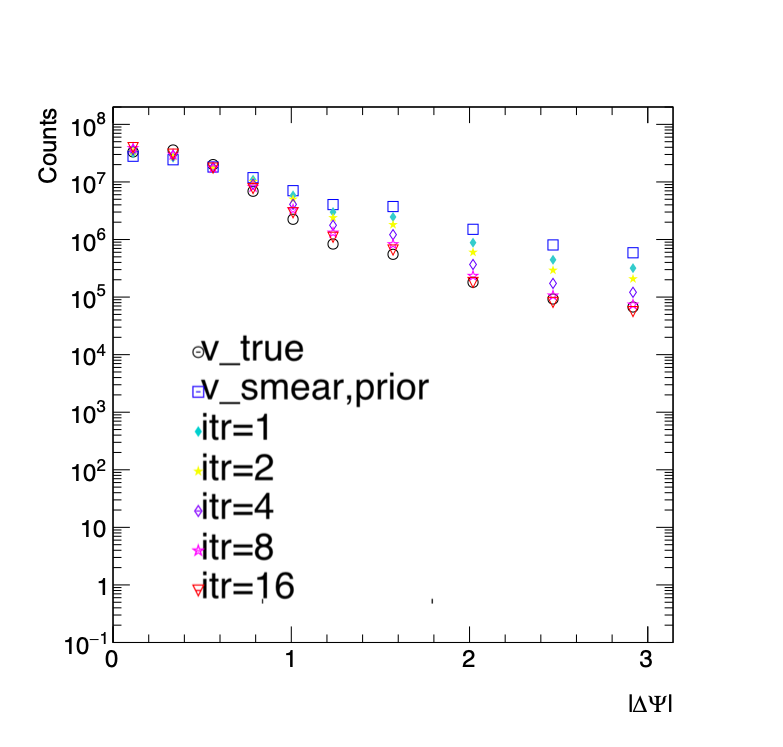
\includegraphics[width=0.3\textwidth]{1d_the.png}}
    \caption{不同的边缘分布在一维的贝叶斯展开结果\label{fig:bu1d}}%
    \end{figure}
    可以看出,在一维上,随着迭代的进行,各边缘分布都呈现了收敛趋势。但是,仅仅$16$次迭代还不足以让迭代结果收敛至真实分布概率较低区域。
    \item 二维边缘分布:\par
    我们选取平均模长和夹角大小的联合分布进行研究,该二维联合分布的边缘分布收敛情况如\ref{fig:bu2d}所示。\par
    \begin{figure}[htbp]
    \centering
    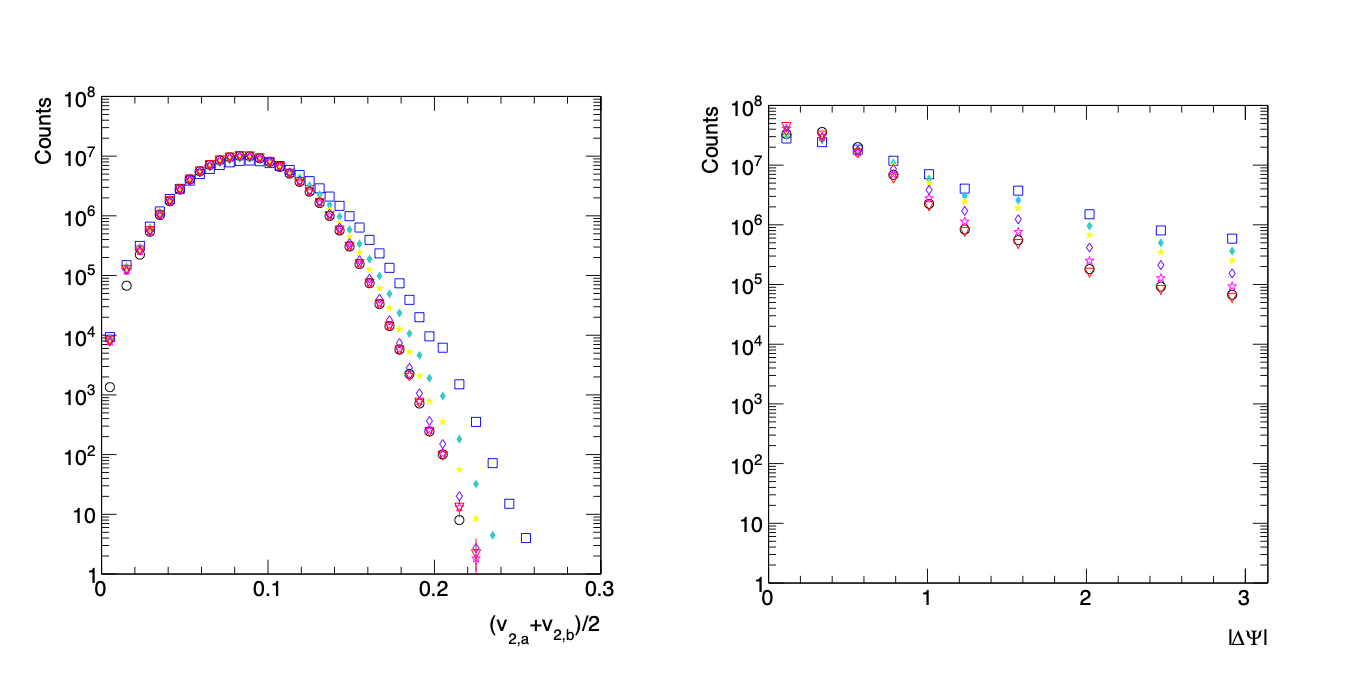
\includegraphics[width=140mm]{2d_vp_the.png}
    \caption{平均模长和夹角大小的联合分布的贝叶斯展开结果\label{fig:bu2d}}%
    \end{figure}
    边缘分步与一维情形类似,而对于联合分布,二维热图更能反应出分布的性质,如图\ref{fig:bu2dc}将迭代结果,真实分布与观测分布进行了对比。可以看出,16次迭代后,联合分布已经可以收敛到与真实分布接近的水平。\par
    \begin{figure}[htbp]
        \centering
        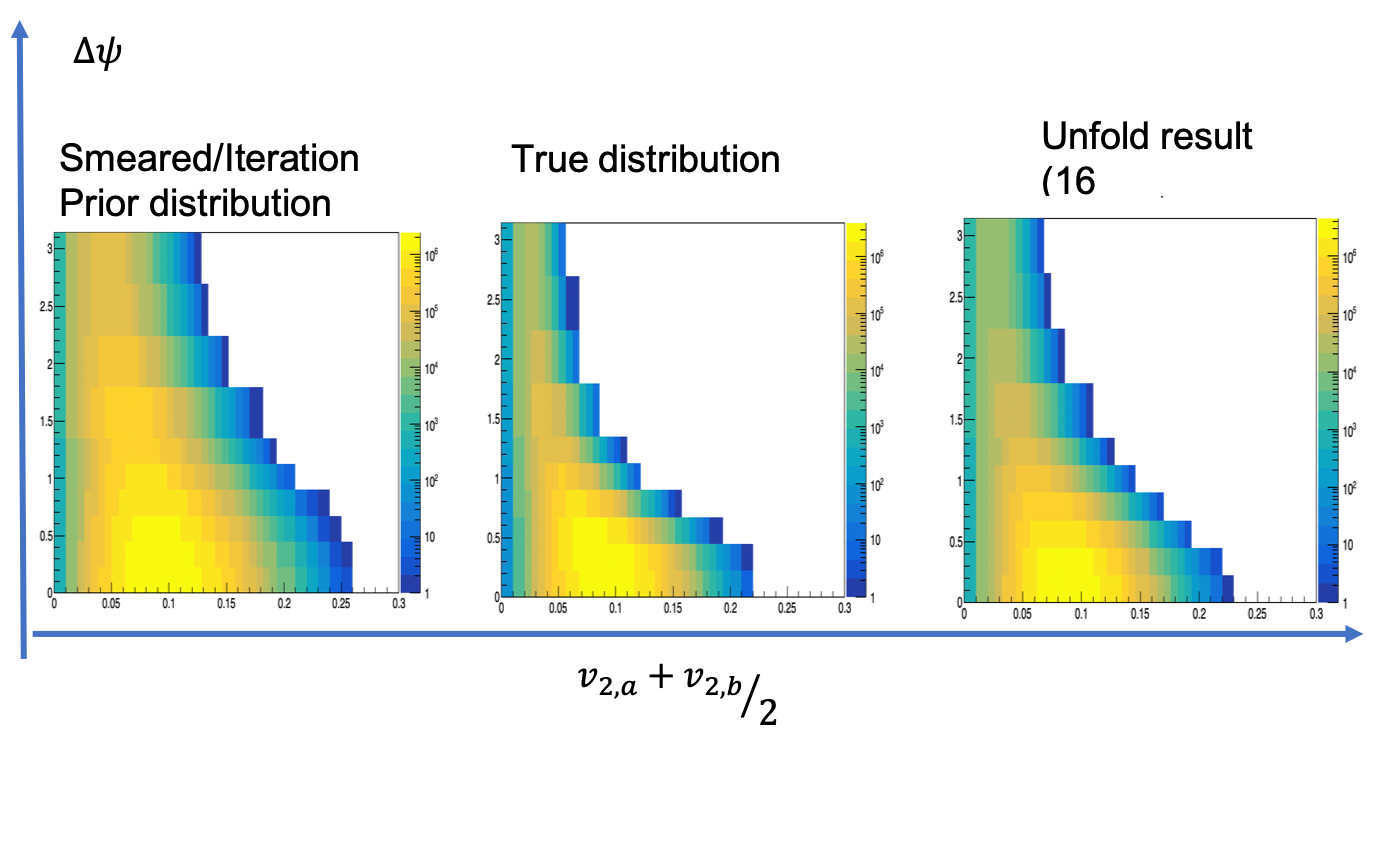
\includegraphics[width=140mm]{2d_vp_the_compare.png}
        \caption{平均模长和夹角大小的联合分布的贝叶斯展开结果\label{fig:bu2dc}}%
        \end{figure}
    热图的缺陷是难以给人以直观的定量感受,因而我们绘制了绝对残差和相对残差的热力图。\ref{fig:res2d}\par
    \begin{figure}[htbp]
        \centering
        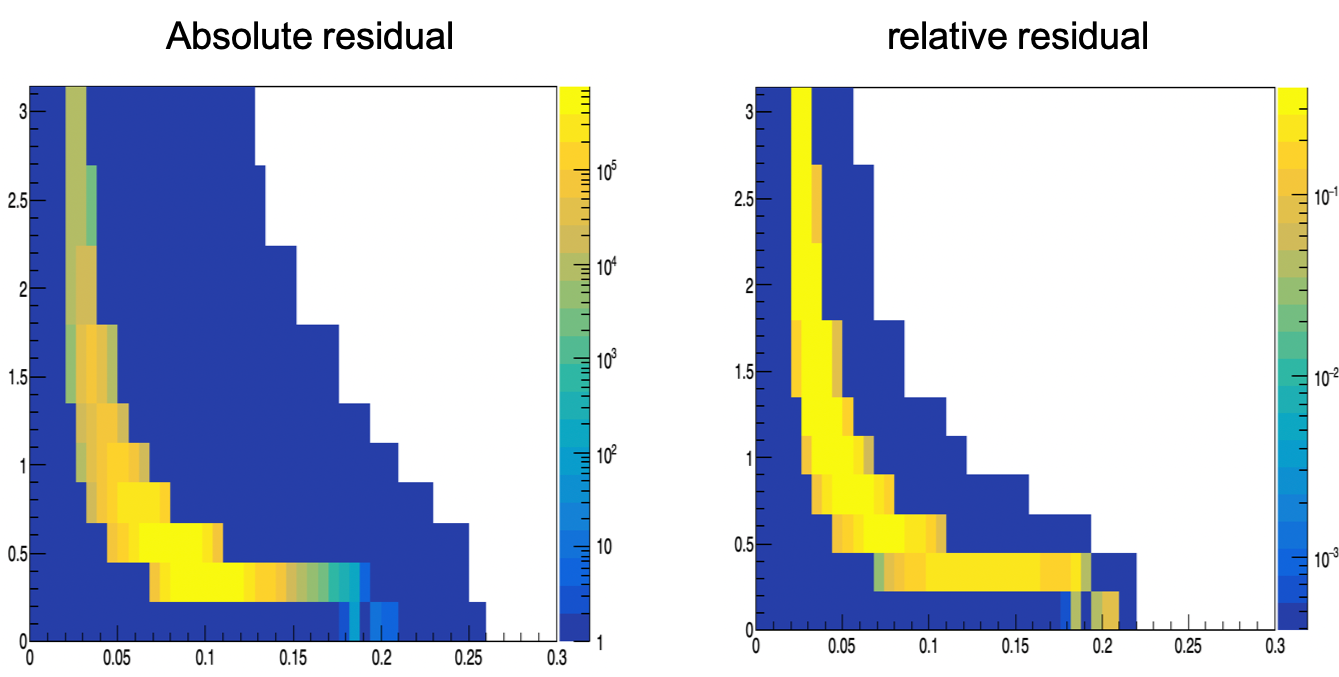
\includegraphics[width=140mm]{res.png}
        \caption{平均模长和夹角大小的联合分布的贝叶斯展开残差结果\label{fig:res2d}}%
        \end{figure}
        从残差的分布来看,随着模长均值的减小,夹角维度分布的弥散收敛逐渐困难,为了观察细节,我们将条件分布矩阵一并画出,如图\ref{fig:resmat}。
        \begin{figure}[htbp]
            \centering
            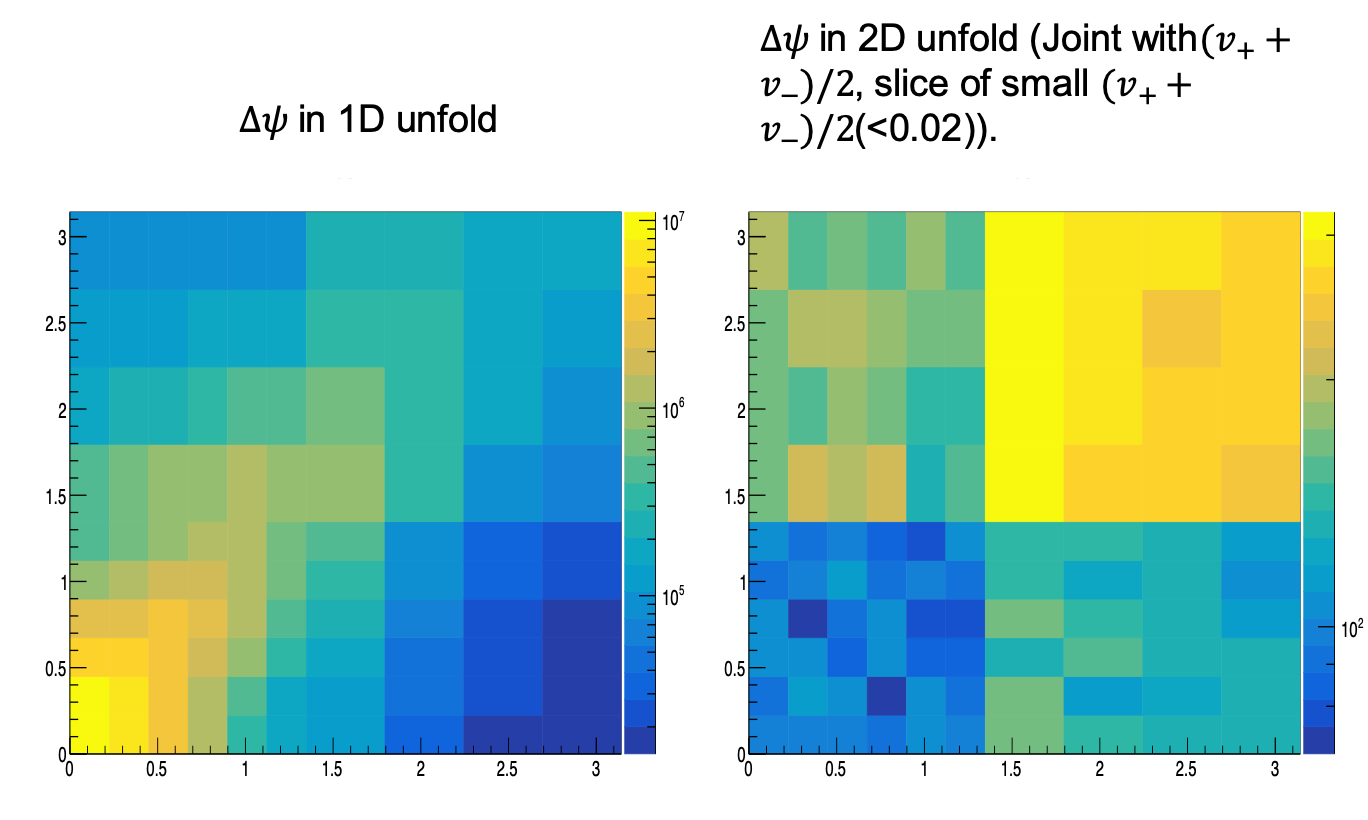
\includegraphics[width=140mm]{resmat.png}
            \caption{夹角大小维度的迁移矩阵\label{fig:resmat}}%
            \end{figure}
        从条件分布矩阵中可以看出,在平均模长较小的区间内,夹角的响应是更宽的(如图\ref{fig:argue}),因而将其还原的操作也势必非常困难。
        \begin{figure}[htbp]
        \centering
        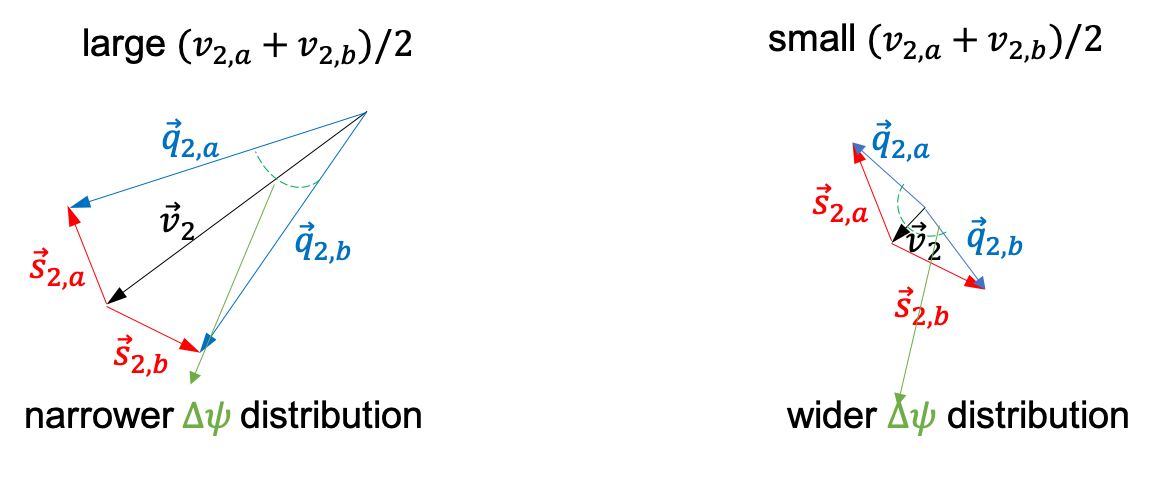
\includegraphics[width=140mm]{argue}
        \caption{不同平均模长下展宽行为\label{fig:argue}}%
        \end{figure}
        \item 三维分布:\par
        将三维分布的结果投影到三个维度,获得边缘分布如图\ref{fig:bu3d}。\par
        \begin{figure}[htbp]
            \centering
            \subfloat[$(v_++v_-)/2$]{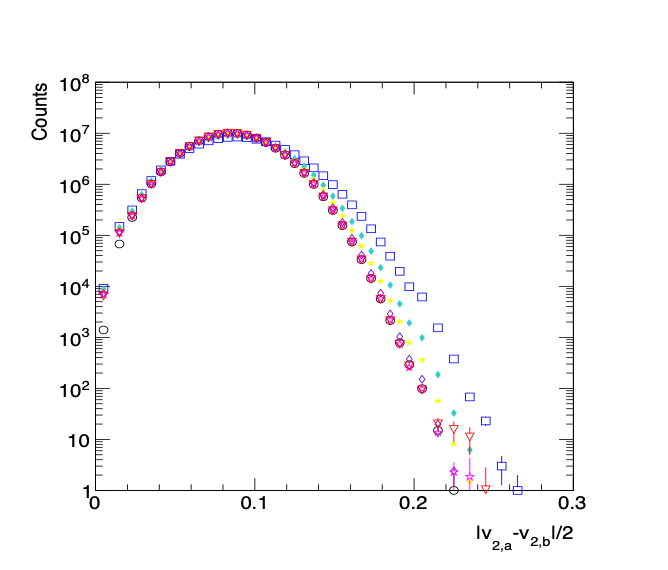
\includegraphics[width=0.3\textwidth]{3d_vp.png}}
            \subfloat[$|v_+-v_-|/2$]{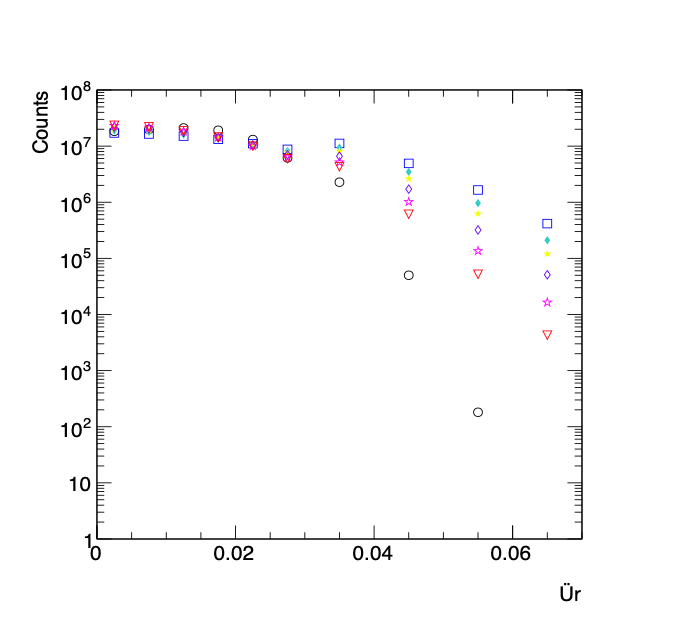
\includegraphics[width=0.3\textwidth]{3d_vm.png}}
            \subfloat[$|\Delta\Psi|$]{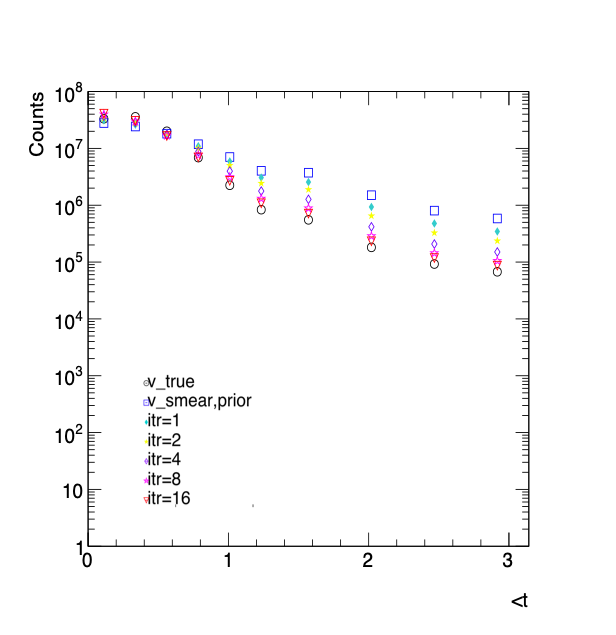
\includegraphics[width=0.3\textwidth]{3d_the.png}}
            \caption{三维的贝叶斯展开结果\label{fig:bu3d}}%
            \end{figure}
        从边缘的分布的收敛行为来看,三维也取得了较好的效果。\par
\end{enumerate}
综上,利用贝叶斯展开,可以对接近真实情形的解关联模型数据进行较好的处理,具有运用到实验数据上的价值。但是,应用到实验数据上时,对于条件分布矩阵的产生,需要
综合理论模型进行更好的设计。

\section{结论}
在流与非流事件的分类课题中,我们采用了主成分分析和神经网络两种方法进行了尝试。其中主成分分析方法
可以在定性上给出流与非流事件的区别,并且能够直观的显示出流与非流事件区别的形式;而神经网络方法在训练集足够充分的情况下,能够很好的区分流与非流事件,并且只要
事件平均数达到一定数据,均可以得到很高的准确度。但是,要验证我们所用的机器学习的方法是否
真正合理,接下来势必要用真实的实验数据进行测试。\par
在利用神经网络拟合相对论性重离子碰撞的课题中,我们所采用的贝叶斯神经网络,通过末态粒子观测量,可以对相对论性重离子碰撞过程的演化参数给出较好的拟合。在一步的研究过程中,一方面可以利用贝叶斯神经网络的特性
给出置信区间,另一方面还需要进行更多的计算进行验证。\par
在利用贝叶斯展开研究集体流长程解关联效应的课题中,通过简化模型,我们验证了贝叶斯展开在这一问题中的有效性与实用价值。在进一步的研究中,我们将结合理论模型,将贝叶斯展开这一工具应用于实验数据中,对实际的解关联现象进行研究。
\section{致谢}
非常感谢宋慧超老师选择的富有创新性和挑战性的课题,并且在本研期间给予我们的诸多帮助和谆谆教诲。同时也要感谢组内的各位成员,
尤其是赵文斌、黄恒丰以及刘楚源,在本研期间帮助我们产生了所需要的数据以及指导我们如何使用这些数据,
也感谢刘子鸣和鄢语轩同学的热情讨论和建议。同时也感谢美国纽约州立大学石溪分校的贾江涌老师和丹麦哥本哈根大学尼尔斯玻尔研究所的周铀老师的暑期指导。

\bibliographystyle{plain}
\bibliography{yinyong2}
%\bibliography{PhysRevD.94.112002}
%\bibliography{PhysRevA.96.042113}
%\bibliography{2017arXiv170300670S}
%\bibliography{2013PhDT........31Q}
%\bibliography{2010LanB...23..240H}
%\bibliography{PhysRevC.58.1671}
%\bibliography{PhysRevC.96.024908}
%\bibliography{PhysRevC.72.064901}
%\bibliography{S0010465514002537}
%\bibliography{PhysRevD.44.3501}
%\bibliography{10.1007_JHEP05(2018)006}
%\bibliography{S037026931630747X}
%\bibliography{10.1007_JHEP02(2016)156}
%\bibliography{PhysRevLett.116.172302}
%\bibliography{PhysRevC.89.064910}



\section{\heiti\zihao{-4}作者简介}
方永康,男,1998年11月出生于安徽省长丰县,2016年从安徽省合肥一六八中学考入北京大学物理学院。\par
钱思天,男,1998年4月出生于安徽省合肥市,2016年从安徽省合肥一六八中学考入北京大学物理学院。
\section{\heiti\zihao{-4}感悟与寄语}
通过本研的经历,初步体验到了研究工作者的经历。在研究过程中总是有苦有乐的,有趣的是可以接触到
之前从未接触到的问题,并且可以尝试用不同的方法进行研究,同时可以和其他人进行交流,共同探讨同一个问题,
进行思想上的碰撞,但研究过程本身是苦的,经常是很长时间内看不到什么进展,所用的方法最终发现存在缺陷而必须改变
方法,或者加一些额外的约束使方法可以适用。总而言之,本科生科研是我们本科生期间一次非常有意义的工作,
在这项工作中,我们结识了许多人,见识了许多新事物,希望在今后我们仍旧可以在学术研究的道路上不断前行。

\section{\heiti\zihao{-4}指导老师简介}
宋慧超,女,北京大学物理学院理论物理研究所研究员,于2009年8月在美国俄亥俄州立大学获得了物理学博士学位。取得博士学位后,先后在美国劳伦斯伯克利国家实验室和俄亥俄州立大学做博士后研究。自2012年10月起,任北京大学物理学院研究员。研究方向是相对论重离子碰撞和夸克胶子等离子体。发表论文20余篇,总引用率超过1700次。获2011年度美国物理学会原子核物理最佳博士论文奖,并于2013年入选青年千人计划。
目前,研究主要集中于以下几个方向:一、夸克胶子等离子体的输运性质;二、QCD 相变临界点附近的长程关联和涨落;三、流体力学模型,耦合模型及临界点附近的动力学模型。


\end{document}
